\documentclass[10pt,conference]{IEEEtran}
\usepackage{cite}
\usepackage{amsmath,amssymb,amsfonts}
\usepackage{algorithmic}
\usepackage{graphicx}
\usepackage{textcomp}
\usepackage{xcolor}
\usepackage[hyphens]{url}
\usepackage{hyperref}
\usepackage{booktabs}
\usepackage{colortbl,pifont,makecell}
\usepackage{pgfplots}
\usepackage{todonotes}
\usepackage{comment}
\pgfplotsset{compat=1.18}

% Ensure letter paper
 \pdfpagewidth=8.5in
\pdfpageheight=11in

% Tighter spacing around floats, captions and displayed equations
% (IEEEtran defaults: textfloatsep 18.6pt, floatsep/intextsep 10.2pt,
% abovecaptionskip 6pt, display skips 6.75pt).
\setlength{\textfloatsep}{8pt plus 2pt minus 2pt}
\setlength{\dbltextfloatsep}{8pt plus 2pt minus 2pt}
\setlength{\floatsep}{6pt plus 1pt minus 1pt}
\setlength{\dblfloatsep}{6pt plus 1pt minus 1pt}
\setlength{\intextsep}{6pt plus 1pt minus 1pt}
\setlength{\abovecaptionskip}{3pt}
\setlength{\belowcaptionskip}{2pt}
% \normalsize resets the display skips every time it runs, so extend it.
\makeatletter
\g@addto@macro\normalsize{%
  \setlength{\abovedisplayskip}{3pt plus 2pt minus 1pt}%
  \setlength{\belowdisplayskip}{3pt plus 2pt minus 1pt}%
  \setlength{\abovedisplayshortskip}{0pt plus 2pt}%
  \setlength{\belowdisplayshortskip}{3pt plus 2pt minus 1pt}}
\makeatother

% Cells of the related-work comparison table
\newcommand{\cyes}{\ding{51}~\textbf{Yes}}
\newcommand{\cno}{\ding{55}~No}
\newcommand{\cpartial}{$\triangle$~Partial}

% Highlighted answer / takeaway box: full column width, light-grey fill, thin frame,
% bold label, italic text. Usage: \answerbox{Answer \#1 for Q1}{One sentence.}
\newcommand{\answerbox}[2]{\par\vspace{3pt}\noindent
  \fcolorbox{black}{gray!15}{\parbox{\dimexpr\linewidth-2\fboxsep-2\fboxrule\relax}{\textbf{#1:} \textit{#2}}}\par\vspace{3pt}}


%%%%%%%%%%%%%%%%%%%%%%%%%%%%%%%%%%%%%%%%
%%%%%%%%%%%%%%% -- TITLE -- %%%%%%%%%%%%%%%
\title{FourShadow: 
Investigating SIMT Tensor Core Scaling Across Hierarchies of a RISC-V GPU}
%Scaling Across Multiple RISC-V GPU Hierarchies}
%Scaling Across RISC-V GPU Design Parameters}
% alt: FourCast, FourSight
%%%%%%%%%%%%%%%%%%%%%%%%%%%%%%%%%%%%%%%%

%%%%%%%%%%%%%%%%%%%%%%%%%%%%%%%%%%%%%%%%
%%%%%%%%%%%%% -- AUTHORS -- %%%%%%%%%%%%%%
% ISPASS 2027 reviews double-blind: no author names or affiliations in the submission.
\author{\IEEEauthorblockN{Anonymous Author(s)}}
%%%%%%%%%%%%%%%%%%%%%%%%%%%%%%%%%%%%%%%%

\begin{document}
\maketitle
% ISPASS requires numbered pages; IEEEtran's conference mode prints none by default.
\thispagestyle{plain}
\pagestyle{plain}

%%%%%%%%%%%%%%%%%%%%%%%%%%%%%%%%%%%%%%%%
%%%%%%%% -- PAPER CONTENT STARTS -- %%%%%%%%%

\begin{abstract}
Tensor cores supply most of a GPU's arithmetic throughput, and each NVIDIA generation has bought more of it with silicon: from the V100 to the B200, dense FP16 tensor throughput grew from 125 to 2,200 TFLOPS, while throughput per transistor rose only 1.8$\times$. Whether a tensor-core feature is worth its silicon therefore depends on its microarchitecture, yet NVIDIA documents what each feature delivers, not how, and shipped silicon cannot be reconfigured to measure the effect of a design parameter. This paper presents FourShadow, the white-box counterpart of a commercial tensor core: an open, synthesizable tensor-core microarchitecture on the RISC-V Vortex GPGPU that implements warp-group MMA and 2:4 structured sparsity with internals that can be read and changed. Where FourShadow agrees with an RTX 5080 and an H100, its mechanism explains theirs: a warp-group MMA waits for its shared-memory $A$ operand on every instruction, a fixed delay independent of the tile width, and 2:4 sparsity halves only part of a GEMM's per-$K$ cost, a part that shrinks as the tile widens. Sweeping FourShadow shows that per-lane throughput peaks at 16 threads per warp and that a wider warpgroup speeds up the warp-group MMA but not the rest of the kernel, which the core's instruction front end limits. On an AMD Alveo U55C FPGA at 250\,MHz, warp-group MMA speeds up Llama~2 prefill by 10.18$\times$ and decode by 7.76$\times$ end to end over the dense base tensor core.
\end{abstract}

\section{Introduction}
\label{sec:intro}
\begingroup\renewcommand{\thefootnote}{}\footnotetext{The first two authors contributed equally to this work. Artifact: we will release the FourShadow RTL, simulator, kernels and the scripts that produce every figure in a public GitHub repository; its URL will appear in the camera-ready version if accepted.}\endgroup

Tensor Cores~\cite{nvidia2017volta, nvidia2020ampere, nvidia2022hopper, nvidia2024blackwell} and Matrix Cores~\cite{amd2020cdna1, amd2021cdna2, amd2023cdna3, amd2025cdna4} carry the AI throughput of modern GPUs: they execute matrix multiply-accumulate (MMA) operations at far higher throughput than the SIMT pipelines beside them. Unlike the systolic arrays of standalone accelerators such as Google's TPUs~\cite{jouppi2017indatacenterperformanceanalysistensor, jouppi2020domain, norrie2021design, jouppi2021ten, jouppi2023tpuv4} and AWS Trainium~\cite{aws_trainium_architecture}, a GPU tensor core is a functional unit of the SIMT core. Each generation has raised its throughput with larger MMA tiles, MMA instructions shared by the four warps of a warpgroup, operands read from shared memory~\cite{luo2025dissectingnvidiahopperarchitecture}, and 2:4 structured sparsity~\cite{nvidia2020ampere, mishra2021acceleratingsparsedeepneural}.

This throughput has been bought with silicon, and since Dennard scaling ended~\cite{hennessy2019golden}, silicon also costs power: the energy efficiency of transistors no longer keeps pace with their number~\cite{esmaeilzadeh2011dark}. From the V100 to the B200, NVIDIA's dense FP16 tensor throughput grew from 125 to 2,200 TFLOPS, while the transistor count grew from 21.1 to 208 billion and the board power from 300 to 1,000\,W~\cite{nvidia2017volta, nvidia2024blackwell}. Throughput per transistor thus rose only about 1.8$\times$, from 5.9 to 10.6 TFLOPS per billion transistors, so most of the gain came from more silicon. Every tensor-core feature, from larger tiles and the operand buffers of warp-group MMA to the sparsity datapath and its metadata, adds area. Whether a feature or design point is worth its silicon is therefore a question of area efficiency: the performance it delivers per unit area.

Judging this efficiency requires answers to two questions, which organize this paper. \textbf{Q1: What is the microarchitectural behavior behind NVIDIA's tensor-core features?} Vendor documents and microbenchmarks report what each feature delivers, not the mechanism that produces it. NVIDIA's PTX ISA defines what a sparse MMA instruction computes and gives it a metadata operand that marks the kept values~\cite{nvidia2026ptxisa}, and microbenchmarks measure the throughput of such instructions on a Hopper GPU~\cite{luo2025dissectingnvidiahopperarchitecture}; neither says which part of a GEMM's work sparsity removes or what loading the metadata costs. \textbf{Q2: How does a tensor core behave as its architectural parameters change?} A commercial GPU ships one point of the design space, with its threads per warp and issue width fixed in silicon; the design points around it are unmeasured, and so is whether that point is the best one.

Current platforms answer neither question. Microbenchmarking studies of NVIDIA Tensor Cores~\cite{jia2018dissectingnvidiavoltagpu, raihan2019modeling, markidis2018tensorcore, martineau2019v100, jia2019dissectingnvidiaturingt4, yan2020demystifying, 9926299, 9931992, 10579250, luo2025dissectingnvidiahopperarchitecture, 10.1145/3725843.3756041, 11575375} and AMD Matrix Cores~\cite{10590025, kurzynski2025mfma, jarmusch2026microbenchmark} measure shipped silicon, so they cannot change the organization behind an outcome, and NVIDIA's documents give the area and power of the whole GPU only~\cite{nvidia2017volta, nvidia2020ampere, nvidia2022hopper, nvidia2024blackwell}. Simulators abstract the tensor core: Accel-Sim~\cite{accel-sim} models a tensor-core instruction by a latency and an initiation interval, GPGPU-Sim~\cite{raihan2019modeling} has no sparsity, and both fix the warp at 32 threads and have no RTL. Tensor cores built on the open Vortex GPU each lack a piece (Section~\ref{sec:related}, Table~\ref{tab:related_work_comparison}): Virgo~\cite{kim2025virgo} and CoopWarp~\cite{nada2025cooperative} have neither warp-group MMA nor sparsity, CoopWarp exists only in a simulator, and Ten-Four~\cite{rout2026tenfouropensourcefuseddot} is a dot-product unit rather than a tensor core; the tensor-core extensions RM-STC~\cite{huang2023rmstc}, VEGETA~\cite{jeong2023vegeta}, Sparse TC~\cite{zhu2019sparsetensorcore} and SIMD$^2$~\cite{zhang2022simd2} have no warp-group MMA and no open source. No prior platform combines configurable threads per warp and issue width, warp-group MMA, 2:4 sparsity, and both synthesizable RTL and a cycle-level simulator.

To this end, this paper presents \textit{\textbf{FourShadow}}, the white-box counterpart of a commercial tensor core, built on the open-source RISC-V Vortex GPGPU~\cite{vortex}: it implements the same features with internals that can be read and changed (Figure~\ref{fig:figure_integration}). FourShadow is an open, synthesizable and reconfigurable tensor-core microarchitecture that obtains the causes by design-space exploration, changing one microarchitectural parameter at a time. The name has two meanings. As a \emph{shadow}, it outlines an object that cannot be inspected, in four components: the base tensor core, the warp-group tensor core, the sparse tensor core and the programming model. We measure it beside an RTX 5080 and an H100 to answer Q1: where the two agree, the mechanism visible in FourShadow is a candidate explanation; where they differ, the difference excludes one. As a \emph{foreshadow}, being reconfigurable, it foretells the trends of design points that no commercial GPU ships, which answers Q2; its best point carries over to a commercial design only as far as the two match. Threads per warp, issue width, accumulator registers, operand staging, dot-product length and data format are build parameters. Performance is measured in cycles on SimX and end to end on an FPGA, and area by ASIC synthesis in ASAP7.

Building these features on RISC-V is not a port of NVIDIA's design, because the RISC-V instruction set sets the limits. Its 32 floating-point registers per thread give $A$, $B$ and the accumulator eight each, so the tile shape follows this budget and the threads per warp. An MMA micro-operation names four registers, for $A$, $B$, $C$ and $D$, so the doubled $B$ operand of a sparse MMA fits in its one $B$ register only in some configurations, the asymmetric ones, and not in the symmetric ones. Warp-group MMA needs shared-memory descriptors and a tile buffer shared by the independently advancing warps of a warpgroup, and the 2:4 metadata needs its own load instruction. Section~\ref{sec:design} presents these solutions.

FourShadow answers both questions. For Q2, per-lane warp-group MMA throughput peaks at 16 threads per warp, and NVIDIA's 32 threads sit on that plateau (Section~\ref{sec:eval_threads}).
A wider warpgroup speeds up the warp-group MMA but not the rest of the kernel, which the core's instruction front end limits (Section~\ref{sec:eval_iw}). For warp-level MMA, sparsity speeds up the asymmetric configurations more than the symmetric ones (Section~\ref{sec:eval_sparse_sym}). For Q1, 2:4 sparsity halves only part of a GEMM's work (Section~\ref{sec:eval_sparse_halves}), and for warp-group MMA that part shrinks as the tile widens, on FourShadow and an H100 alike (Section~\ref{sec:eval_sparse_wg}). Only a reconfigurable white-box design can measure these: a shipped GPU fixes its threads per warp, issue width and operand staging and gives no area of its tensor cores, and a simulator has no tensor-core organization to vary and no RTL to synthesize.

In summary, this paper makes the following contributions:

\begin{itemize}
    \item We build FourShadow, an open-source, synthesizable tensor-core framework on the RISC-V Vortex GPGPU, with warp-group MMA in register/shared-memory (RS) and shared-memory/shared-memory (SS) operand staging and a 2:4 structured-sparsity datapath (Section~\ref{sec:design}).

    \item We answer Q2 by sweeping threads per warp and issue width: per-lane throughput peaks at 16 threads, and the core's instruction front end limits a wider warpgroup (Section~\ref{sec:eval_hierarchy}).

    \item We answer Q1 by measuring FourShadow beside an RTX 5080 and an H100: the share of the per-$K$ cost that sparsity halves bounds the sparse speedup, and it falls as the warp-group tile widens (Section~\ref{sec:eval_sparse}).

    \item We report RISC-V design findings: the sparse speedup depends on symmetric versus asymmetric configurations, a 2K-wide FEDP outweighs its deeper pipeline, and accumulator capacity likely explains WMMA's gap to WGMMA on Hopper (Sections~\ref{sec:eval_wgmma} and~\ref{sec:eval_sparse_sym}).

    \item We validate FourShadow by FPGA implementation and ASIC synthesis. On an AMD Alveo U55C FPGA at 200\,MHz, WGMMA speeds up Llama-3.2-1B prefill and decode end to end by $10.18\times$ and $7.76\times$ over the dense base tensor core, and with 2:4 sparsity added by $12.39\times$ and $8.57\times$ (Sections~\ref{sec:eval_fpga} and~\ref{sec:eval_asic}).%; the combined extensions reach $12.74\times$ on MoE.
\end{itemize}

\section{Background}
\label{sec:background}
% Sources (read-only): 00_doc/ispass_direction/riscv_vs_nvidia/PRELIM_REPORT.md (sections 3.1-3.5, 5) and web_facts.md (main);
% 00_doc/vortex-wgdxa2k/results/RISCV_VS_NVIDIA_VORTEX_SIDE.md (part4; SimX/LLVM on pinned d6426cca1);
% 02_nvidia/runs/riscv-vs-nvidia-20261118/tables.md, table T1 (part1; RTX 5080 sm_120 measured, sm_90 compile-only);
% 00_doc/ispass_direction/reference_repos.md (Virgo, CoopWarp); Vortex sources in 01_github/vortex-wgdxa2k (pinned) and the
% master README (7300bc849). Never state Vortex vs NVIDIA speed; never say NVIDIA has no scoreboard; never extend the
% Turing/Ampere reverse engineering to Blackwell (PRELIM_REPORT.md section 5).

% P:bg-roadmap
Vortex is the GPU on which this paper builds its tensor cores. This section describes its organization (Section~\ref{sec:bg_hierarchy}), the research that builds on it (Section~\ref{sec:bg_platform}) and how it differs from NVIDIA GPUs (Section~\ref{sec:bg_nvidia}).

\subsection{The Vortex GPU}
\label{sec:bg_hierarchy}

% P:bg-vortex-stack
Vortex~\cite{vortex} is an open-source GPU built on the RISC-V instruction set architecture (ISA). It is released as a full stack: synthesizable SystemVerilog RTL with FPGA and ASIC synthesis flows, a cycle-level simulator, SimX, and an LLVM-based compiler, VOLT~\cite{10.1145/3771775.3786275}, with OpenCL, HIP and Vulkan front ends. A design is typically prototyped in SimX and then implemented in the RTL.
% Sources: master README.md lines 5-7 (full stack; SimX, RTL simulator, Xilinx/Altera FPGAs; prototype in simx before the RTL
% implementation), 44-48 (OpenCL 1.2, Vulkan, HIP), 134 (VOLT); pinned hw/syn/{altera,xilinx,synopsys,yosys} [S].

% P:bg-vortex-hierarchy
A Vortex processor is organized as clusters of sockets, and a socket groups the cores that share the first-level instruction and data caches. Each core is a single-instruction, multiple-thread (SIMT) pipeline that runs $\mathit{NW}$ warps. A warp is a group of $\mathit{NT}$ threads that execute the same instruction on $\mathit{NT}$ lanes of the datapath, so the threads per warp ($\mathit{NT}$) set the width of every per-thread structure: the register file holds $\mathit{NT}$ entries per architectural register, and the load/store unit has $\mathit{NT}$ lanes. The core issues instructions from up to $\mathit{IW}$ warps in the same cycle, its issue width (Section~\ref{sec:bg_issue}). The numbers of clusters, sockets and cores, $\mathit{NT}$, $\mathit{NW}$ and $\mathit{IW}$ are all build-time parameters.
% Sources [S, pinned]: hw/rtl/VX_socket.sv:142-148, 194-196 (I- and D-cache clusters per socket); VX_cluster.sv:211-237 (L2 per
% cluster); VX_config.toml:4-6 (clusters, cores, socket size), 47-55 (NW, NT, issue width, SIMD width = NT), 92 (LSU lanes = SIMD width).

\subsection{Vortex as a Research Platform}
\label{sec:bg_platform}

% P:bg-platform
Because every layer of Vortex is open, prior work uses it in three ways: as a base for new hardware units, as RTL to synthesize, and as a platform for design-space exploration. As a base, Gouk et al.\ embed the RTL of their CXL controller~\cite{gouk2024breaking} in Vortex so that the GPU reaches DRAM and SSD endpoints over CXL~\cite{gouk2025cxlgpu}; Virgo~\cite{kim2025virgo} places the Vortex SIMT core in a Chipyard system-on-chip and adds matrix units at the level of a core cluster; and Ten-Four~\cite{rout2026tenfouropensourcefuseddot} implements a mixed-precision fused dot-product unit for the tensor-core extension of Vortex. As RTL, Vortex scales to 32 cores on an Altera Stratix~10 FPGA~\cite{vortex}, Virgo synthesizes its system in a commercial 16\,nm process to measure power, and Ten-Four reaches a 4-cycle latency at 300\,MHz on an AMD Alveo U55C FPGA. For design-space exploration, CoopWarp~\cite{nada2025cooperative} integrates a tensor core into Vortex and relates its utilization to the GPU's architectural parameters before proposing cooperative warp execution, and Pu et al.~\cite{pu2025warplevel} implement warp-level features in Vortex both in hardware and in software and compare the two.
% Sources: Gouk et al. HotStorage'24 abstract (CXL root ports, controller integrated at the RTL level); Vortex embedding read in the
% CXL-GPU article (arXiv 2506.15601v1, "Integration with the GPU was achieved using Vortex ... where our controller's RTL design was
% embedded"; published in IEEE Micro 45(6)). Virgo arXiv 2408.12073 sections 3, 3.2 (vx_core in Chipyard), 1 and 5 (commercial 16nm,
% active power). Ten-Four arXiv 2512.00053 abstract. Vortex MICRO'21 abstract (32 cores, Stratix 10). CoopWarp HPCA'25 abstract.
% Pu et al. arXiv 2505.03102 abstract (DATE 2025 workshop W05.4.1). Skybox (ASPLOS'23) omitted: its Vortex basis was not readable
% in a primary source.

\subsection{Vortex and NVIDIA GPUs}
\label{sec:bg_nvidia}

% P:bg-nv-frame
Vortex adopts the SIMT programming model of NVIDIA GPUs, with warps, thread blocks, shared memory, barriers, and warp- and warpgroup-level matrix instructions, but not the machine beneath it. The two machines differ in three ways that change how the same kernel source executes: the ISA, the registers per thread and the configurability of the core.
% Sources: web_facts.md section C items 1 and 3 (abstractions borrowed on purpose: tensor_core_wgmma_engine.md:4 "NVIDIA-style warp /
% warpgroup MMA"; MICRO'21 section 3.1 maps PTX warps and CTAs onto Vortex) [S].

% P:bg-nv-isa
\textbf{ISA.} Vortex executes standard RISC-V, RV32IMAF in this paper, and encodes its GPU instructions, such as thread control, tensor-core and asynchronous-copy instructions, in the custom opcode space of RISC-V. NVIDIA compiles CUDA to PTX, a virtual ISA~\cite{nvidia2026ptxisa}, which is translated to the machine ISA, SASS; NVIDIA documents SASS only as per-generation lists of opcodes~\cite{nvidia2026binutils}. A SASS instruction occupies 16 bytes and carries compiler-set stall, yield, dependence-barrier and reuse fields~\cite{10.1145/3725843.3756041}, whereas a Vortex instruction occupies 4 bytes and carries no scheduling field; a per-warp hardware scoreboard resolves hazards instead. NVIDIA's compiler thus encodes part of the instruction timing into the binary, while the timing of Vortex lives entirely in its open RTL and SimX.
% Sources: PRELIM_REPORT.md 3.1 [M: every SASS instruction 16 B on sm_120 and sm_90; every Vortex instruction 4 B, RVC off],
% 3.2 [R: control fields from Huerta et al. on Turing/Ampere; validated by part1 on sm_120 and sm_90 (reuse bits 154,736/154,736,
% stall 4 = 4.06-cycle FFMA latency)]; RISCV_VS_NVIDIA_VORTEX_SIDE.md 1 (-march=rv32imaf, 4 B), 3.1 (custom-0/custom-1), 3.4
% (VX_scoreboard.sv:101, decode.cpp:480-491: no scheduling bits) [S].

% P:bg-nv-registers
\textbf{Registers per thread.} A RISC-V thread has 32 integer and 32 floating-point registers, fixed by the ISA, and Vortex builds the full set for every warp, so a kernel's register use never lowers the number of resident warps. NVIDIA's compiler allocates each thread a per-kernel number of registers, at most 255, from a file of 64K registers per streaming multiprocessor (SM) that all resident warps share~\cite{nvidia2026cudaguide}. Compiled from the same register-tiled GEMM source, in which each thread accumulates a block of the output in registers (its thread tile, Section~\ref{sec:motivation}), NVIDIA's compiler keeps a $16{\times}8$ tile of 128 accumulators without spilling, while the Vortex compiler runs out of its 32 floating-point registers and spills at the $4{\times}4$ tile, as NVIDIA's compiler does when it is limited to 32 registers per thread. The register budget, not the compiler, therefore sets the largest thread tile, and the large register tiles of SIMT kernels on NVIDIA GPUs do not carry over to a RISC-V GPU.
% Sources: [S] VX_gpu_pkg.sv:52-65 (RV_REGS 32, NUM_REGS = 2 x 32), VX_opc_unit.sv:49 (every warp owns all registers);
% PRELIM_REPORT.md 3.3a. [M] 02_nvidia/runs/riscv-vs-nvidia-20261118/tables.md T1: sm_120 16x8 = 255 regs, 0 spill; 4x4 with
% maxrregcount 32 = 160 B spill stores (0 at 2x2); Vortex 4x4 = 29/29 integer and 32/32 FP registers, 48/41 sp loads/stores;
% Vortex 2x2 = 29 integer and 15 of 32 FP registers, but already 11/12 integer sp loads/stores (PRELIM_REPORT T1; the text names the FP file, not the first spill)
% (RISCV_VS_NVIDIA_VORTEX_SIDE.md 1, pinned d6426cca1, LLVM -O3). Motivation (mot-register-reads) owns the spill-driven reads.

% P:bg-nv-config
\textbf{Configurability.} The threads per warp, warps per core and issue width of Vortex are build-time parameters, and this paper builds cores with 4 to 32 threads per warp and issue widths of 1 to 8 (Table~\ref{tab:config}). An NVIDIA warp has 32 threads on every compute capability~\cite{nvidia2026cudaguide}, and each NVIDIA chip fixes the organization of its SM, so every NVIDIA GPU is one design point, whereas Vortex exposes the warp shape itself as a parameter to study.
% Sources: VX_config.toml:47-55 [S]; CUDA Programming Guide 13.5 Table 33 (warp size 32 for every compute capability) [S].

% P:bg-nv-bridge
These differences make an NVIDIA GPU a different machine rather than another configuration of Vortex. We therefore evaluate FourShadow's tensor cores against the SIMT-only Vortex core they extend (Section~\ref{sec:motivation}), not against an NVIDIA GPU.
% TODO(ispass): the Introduction (Q1), tab:config and the evaluation still compare with the RTX 5080 and H100; remove per the ISPASS redirect.

\section{Related Work}
\label{sec:related}
% Sources (primary, read 2026-11-24): Virgo arXiv 2408.12073v2 (ASPLOS'25); CoopWarp HPCA'25 abstract (imec repository; the full
% text is behind "request a copy" and was not read) and the authors' artifact repository BakrN/vortex @ 4f9134cb, read-only clone
% 01_github/coopwarp-vortex (00_doc/ispass_direction/reference_repos.md section 2) [source-derived]; Ten-Four arXiv 2512.00053v4;
% RoadBlock arXiv 2611.08526v1 (PACT'26, 2 pages). Only tensor-core work built on Vortex is compared here (user, 2026-11-24);
% non-Vortex tensor cores and simulators stay in the Introduction.

% P:rel-frame
Tensor cores built on Vortex each extend one level of the GPU: the core cluster, the SIMT core, or the dot-product datapath inside the tensor core. Table~\ref{tab:related_work_comparison} compares them by the threads per warp they support, by whether they exist as RTL and in a cycle-level simulator, and by whether they provide warp-group MMA and 2:4 sparsity.

% P:rel-virgo
Cluster-level matrix units trade flexibility on small matrices for larger operations. Virgo~\cite{kim2025virgo} keeps the Vortex SIMT cores for general computation and adds a Gemmini systolic array to each core cluster, where it reads its operands from shared memory and accumulates in its own memory, so one operation covers the tile of a thread block. Synthesized in a commercial 16\,nm process, Virgo lowers active power by 67.3\% and 24.2\% against Ampere-style and Hopper-style tensor cores coupled to the core, which it also builds in RTL; its Hopper-style tensor core runs an asynchronous MMA that one warp initiates. Virgo evaluates warps of 8 threads, has no sparsity, and takes its cycle counts from RTL simulation rather than from a cycle-level simulator.
% Sources: abstract and section 6.1.2 (67.3% and 24.2% lower active power than the Ampere-style and Hopper-style core-coupled designs);
% section 3 (Vortex SIMT core, Gemmini at the cluster); section 4 ("the indivisible atom of computation is a threadblock- or
% workgroup-level matrix multiplication ... this approach sacrifices flexibility for workloads that use smaller matrix dimensions");
% section 5.1.3 (a warp kicks off the matrix unit via an initiate instruction and later waits); Table 2; artifact appendix A.

% P:rel-coopwarp
A tensor core coupled to the SIMT core receives its operands through the register file, whose capacity and bandwidth limit the size of each operation~\cite{kim2025virgo}. CoopWarp~\cite{nada2025cooperative} integrates such a tensor core into Vortex, relates its utilization to the GPU's architectural parameters, and finds it severely underutilized in many configurations. Its cooperative warp execution lets the warps of a group split the $K$ dimension of a tile and accumulate into one shared tile buffer, which reduces the memory a GEMM needs and reaches 3$\times$ the performance of its baseline tensor core in the best case. Each warp still issues its own MMA, the tensor core takes FP16 inputs and has no sparsity, and it is modeled in SimX only: the repository's standalone tensor-core RTL is not part of the Vortex RTL.
% Sources: HPCA'25 abstract (imec record: integration into Vortex, intrinsics for GEMM kernels, "the tensor core is severely
% under-utilized in many cases", cooperative warp execution "to reduce GEMM memory requirements", "up to 3x" over the baseline tensor
% core). Repository [source-derived]: cooperative_kernel.cpp:80-91 (per-warp tc_mma_acc_buf, vx_barrier, tc_flush_wg),
% sim/simx/tensor_core.cpp:42-75 (FP16 in, FP32 accumulate; other formats throw), K split by WARP_GROUP_SIZE (reference_repos.md),
% tensor_rtl/ standalone (no reference from hw/rtl). Family limit: Virgo section 1 ("restricting operation size due to register file
% capacity and bandwidth constraints").

% P:rel-datapath
Datapath designs improve the arithmetic inside the tensor core. Ten-Four~\cite{rout2026tenfouropensourcefuseddot} is a fused mixed-precision dot-product unit for the tensor-core extension of Vortex: one pipeline multiplies TF32, FP16, BF16, FP8, BF8, INT8, INT4 and microscaling inputs and accumulates in FP32 or INT32. It reaches a 4-cycle latency at 300\,MHz on an AMD Alveo U55C FPGA and runs 2.7$\times$ to 7.9$\times$ faster than units built from the HardFloat and FPnew libraries, at less than 60\% of their area. RoadBlock~\cite{rout2026roadblock} extends Ten-Four to custom microscaling formats and stages their scale factors in a tensor-core SRAM, so that a warp-level MMA can use them without an extra source operand.
% Sources: Ten-Four abstract (formats, OCP MX, 4-cycle latency at 300 MHz on the U55C, "2.7x-7.9x speedup over Berkeley HardFloat and
% FPnew at less than 60% the area cost"), section 3.2; RoadBlock sections 1-2 ("Since Vortex TCU WMMA instructions only expose three
% source operands, MX metadata cannot be supplied as an additional explicit source. RoadBlock instead duplicates registers f8,f9 into
% a lightweight TCU-SRAM").

% float placed late: Table I (moved from the Introduction) renders at the top of the left column of page 5, off the page of Fig. 1
\begin{table}[t]
\centering
\caption{Tensor cores built on the Vortex GPU, all open source.}
\label{tab:related_work_comparison}
\footnotesize
\setlength{\tabcolsep}{3pt}
\renewcommand{\arraystretch}{0.95}
\newcommand{\ty}{\ding{51}}
\newcommand{\tn}{\ding{55}}
\begin{tabular}{@{}l l c c c c c@{}}
\toprule
\textbf{Work} & \textbf{Level} & \makecell{\textbf{Threads}\\\textbf{per warp}} & \textbf{RTL} & \makecell{\textbf{Cycle}\\\textbf{sim.}} & \makecell{\textbf{Warp-}\\\textbf{group}\\\textbf{MMA}} & \makecell{\textbf{2:4}\\\textbf{sparsity}} \\
\midrule
Virgo~\cite{kim2025virgo} & Cluster & 8 & \ty & \tn & \tn & \tn \\
CoopWarp~\cite{nada2025cooperative} & Core & 4--32 & \tn & \ty & \tn & \tn \\
Ten-Four~\cite{rout2026tenfouropensourcefuseddot} & Datapath & 4--32 & \ty & -- & -- & -- \\
\rowcolor{blue!8}
\textbf{FourShadow (Ours)} & Core & 4--32 & \ty & \ty & \ty & \ty \\
\bottomrule
\multicolumn{7}{@{}l}{\scriptsize --: not applicable to a dot-product unit.}
\end{tabular}
\end{table}
% Cells. Virgo: Level = matrix unit at the core cluster (section 3); threads = Table 2 "8 warps/core, 8 lanes/warp" (the Volta-style
% core in its RTL needs a multiple of 8, reference_repos.md section 1); RTL = synthesizable RTL in Chipyard, 16 nm (sections 1, 5.2);
% cycle sim = none: cycles come from RTL simulation (artifact appendix A; its Vortex SimX has no tensor-core model, reference_repos.md);
% warp-group MMA = none: its Hopper-style baseline is initiated by one warp (section 5.1.3); sparsity = none.
% CoopWarp: Level = core-coupled tensor core in SimX (abstract; sim/simx/tensor_core.cpp); threads = experiments.zip th4/th8/th16/th32;
% RTL = none in the Vortex RTL (tensor_rtl/ is standalone, not referenced from hw/rtl); warp-group MMA = none: each warp issues its own
% MMA into a shared accumulator buffer (cooperative_kernel.cpp:80-91); sparsity = none (grep). [source-derived]
% Ten-Four: Level = fused dot-product unit (title, abstract); threads = four-element FEDP at 4/8 and eight-element at 16/32 threads
% per warp (section 3.2, Table 4 notes); RTL = SystemVerilog, U55C FPGA and ASAP7 (sections 4.5, 4.6); "--" for the tensor-core
% columns: its own sparsity is sparse-lane clock gating (section 3.5), and the 2:4 sparsity and warp-group MMA micro-ops it mentions
% belong to the tensor core it is part of.

% P:rel-fourshadow
FourShadow builds the tensor-core organization around this datapath, and Ten-Four is its dot-product unit (Section~\ref{sec:bg_tcu}). It adds warp-group MMA with register and shared-memory operand staging and 2:4 structured sparsity for both warp-level and warp-group MMA, implements them in the RTL and in SimX, and keeps the threads per warp and the issue width as build parameters (Table~\ref{tab:related_work_comparison}).

\section{FourShadow Design}
\label{sec:design}

This section first describes the base tensor core that FourShadow extends and the concepts it depends on, the issue width with its warpgroups and shared memory (Sections~\ref{sec:bg_tcu}--\ref{sec:bg_smem}), and then FourShadow (Sections~\ref{sec:design_overview}--\ref{sec:design_pm}).

\subsection{Base Tensor Core}
\label{sec:bg_tcu}


The base tensor core is the Tensor Core Unit (TCU), a functional unit in the execute stage of each core beside the ALU, FPU, LSU and SFU (Figure~\ref{fig:figure_integration}). It shares the core's front end, register file, shared memory and caches with those units, and it executes the warp-level matrix multiply-accumulate (WMMA) instruction.

WMMA computes $D = AB + C$, where $A$ is an $M{\times}K$ matrix, $B$ is a $K{\times}N$ matrix, and $C$ and $D$ are $M{\times}N$ matrices. The TCU's compute engine consists of a grid of Fused Dot Product (FEDP) units, each of which computes one output element:
\begin{equation}
\label{eq:fedp}
D_{m,n} =
\sum_{i=0}^{K-1}
\left(A_{m,i} \times B_{i,n}\right) + C_{m,n}.
\end{equation}



A WMMA instruction operates on a \emph{tile}, which is divided into smaller \emph{blocks} to fit the $\mathit{NT}$ FEDP units. Each \emph{micro-op} processes one block, accumulating partial results along the $K$ dimension.
Figure~\ref{fig:tiling_equations} derives the tile dimensions, block dimensions, and number of micro-ops from the threads per warp $\mathit{NT}$; $\mathit{NT}{=}8$ is the running example.


\begin{figure}[ht]
\small
\hrule
\vspace{3pt}
{\raggedright\textit{Given:}\ $M,\,N,\,K$} \\
{\raggedright $\mathit{Number of Threads (NT)=\{2, 4, 8, 16, 32\}}$ } \\ 
{\raggedright $\mathit{Number of Registers (NR)}{=}8$\par}
\centering\textbf{\textsc{Tile (per-warp work chunk)}}
\begin{flalign}
&\mathit{tile\_cap} = \mathit{NT} \!\times\! \mathit{NR},\quad
\ell_g = \lfloor\log_2(\mathit{tile\_cap})\rfloor & \\
&\mathit{xtileM} = 2^{\,\ell_g - \lfloor\ell_g/2\rfloor},\quad
\mathit{xtileN} = 2^{\,\lfloor\ell_g/2\rfloor} & \\
&\mathit{xtileK} = \tfrac{\mathit{tile\_cap}}{\max(\mathit{xtileM},\,\mathit{xtileN})} & \\
&\mathit{tileK} = \mathit{xtileK}\!\times\!\tfrac{4}{\mathrm{sizeof}(\texttt{input\_dtype})} &
\end{flalign}
\noindent\textbf{\textsc{Block (one micro-op)}}
\begin{flalign}
&\mathit{block\_cap} = \mathit{NT},\quad
\ell_b = \lfloor\log_2(\mathit{block\_cap})\rfloor & \label{eq:block_cap}\\
&\mathit{tcM} = 2^{\,\ell_b - \lfloor\ell_b/2\rfloor},\;\;
\mathit{tcN} = 2^{\,\lfloor\ell_b/2\rfloor},\;\;
\mathit{tcK} = \tfrac{\mathit{block\_cap}}{\max(\mathit{tcM},\,\mathit{tcN})} & \label{eq:block_tc}
\end{flalign}
\hrule
\vspace{3pt}
\noindent\textbf{\textsc{Steps (micro-ops per tile)}}
\begin{flalign}
&m_{\mathrm{steps}} = \tfrac{\mathit{xtileM}}{\mathit{tcM}},\quad
n_{\mathrm{steps}} = \tfrac{\mathit{xtileN}}{\mathit{tcN}},\quad
k_{\mathrm{steps}} = \tfrac{\mathit{xtileK}}{\mathit{tcK}} &
\end{flalign}
\hrule
\vspace{3pt}
{\centering\textbf{\textsc{micro-ops per \texttt{mma\_sync}}}\par}
{\raggedright
\noindent\hspace{0.5em}\textbf{for} $\;0$ \textbf{to} $k_{\mathrm{steps}}{-}1$:\\
\hspace{2em}\textbf{for} $\;0$ \textbf{to} $m_{\mathrm{steps}}{-}1$:\\
\hspace{3.5em}\textbf{for} $\;0$ \textbf{to} $n_{\mathrm{steps}}{-}1$:\\
\hspace{5em}one micro-op: $\mathit{tcM}{\times}\mathit{tcN}{\times}\mathit{tcK}$ dot-product
\par}
\hrule
\caption{Tensor-core tiling and micro-op decomposition derived from thread count~$\mathit{NT}$ and register budget~$\mathit{NR}$.}
\label{fig:tiling_equations}
\end{figure}

\textbf{Matrix-Register Mapping:}
Vortex's RV32 ISA provides 32 floating-point registers per thread. The base tensor core uses 24 of them, $\mathit{NR}{=}8$ each for matrices $A$, $B$ and the accumulator $C/D$. A register holds $\mathit{NT}$ 32-bit entries, so each matrix has a budget of $\mathit{NT}{\times}\mathit{NR}$ words. A \emph{tile} is the part of each matrix that one WMMA instruction covers within this budget (the Tile equations of Figure~\ref{fig:tiling_equations}). Panels (a) and (b) of Figure~\ref{fig:figure_register_mapping} show in green how the eight registers of each matrix cover the $8{\times}8{\times}8$ tile ($M{\times}N{\times}K$) of $\mathit{NT}{=}8$ and the $8{\times}4{\times}4$ tile of $\mathit{NT}{=}4$. A 32-bit entry packs two 16-bit or four 8-bit inputs, so a tile covers that many times more elements of $K$ ($\mathit{tileK}$, the last Tile equation).

\begin{figure}[ht]
    \centering
    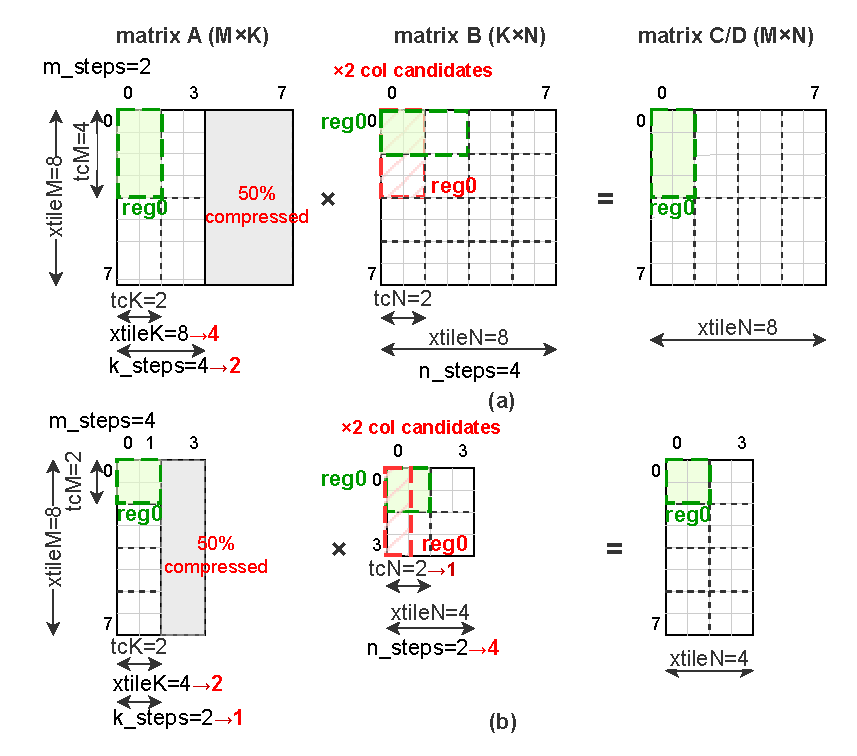
\includegraphics[width=\columnwidth,trim=19 9 13 10,clip]{hpca2027-latex-template/fig/tcu_matrix_register_mapping_sparse_v4_ab_noframe.pdf}
    \caption{Matrix-to-register mapping and tiling for (a) 8-thread and (b) 4-thread configurations (green: dense, red: sparse).}
    \label{fig:figure_register_mapping}
\end{figure}

\textbf{Thread-FEDP Mapping:}
A \emph{block} is the part of a tile that one \emph{micro-op} computes on the $\mathit{NT}$ FEDP units (the Block equations of Figure~\ref{fig:tiling_equations}): the units form a $\mathit{tcM}{\times}\mathit{tcN}$ grid, and each takes a dot product of $\mathit{tcK}$ words. The block is $4{\times}2{\times}2$ for $\mathit{NT}{=}8$ and $2{\times}2{\times}2$ for $\mathit{NT}{=}4$; for $\mathit{NT}{=}32$ it is $8{\times}4{\times}4$ for 32-bit inputs, $8{\times}4{\times}8$ for 16-bit inputs and $8{\times}4{\times}16$ for 8-bit inputs. A configuration is \emph{asymmetric} when a block of $B$ occupies half a register, so that two adjacent blocks pack into one register ($\mathit{NT}{\in}\{2,\allowbreak 8,\allowbreak 32\}$; panel (a)), and \emph{symmetric} when a block of $B$ fills a whole register ($\mathit{NT}{\in}\{4,16\}$; panel (b)). 
The \emph{steps} count blocks per tile along each dimension. For $\mathit{NT}{=}8$, the $8{\times}8{\times}8$ tile and $4{\times}2{\times}2$ block yield $(m_{\mathrm{steps}},n_{\mathrm{steps}},k_{\mathrm{steps}})=(2,4,4)$, requiring 32 micro-ops. These execute with $n$ innermost, $m$ in the middle and $k$ outermost (Figure~\ref{fig:tiling_equations}); $\mathit{NT}{=}4$ requires 16 micro-ops.


\textbf{FEDP Microarchitecture \& Datatypes:}\label{para:datatypes-fedp} The FEDP unit is Ten-Four~\cite{rout2026tenfouropensourcefuseddot}, a four-stage, four-cycle implementation that multiplies, aligns, accumulates, and then normalizes and rounds dot-product results. It multiplies TF32, FP16, BF16, FP8 (E4M3), BF8 (E5M2), INT8 and INT4 inputs and accumulates in FP32 or INT32; each input format is enabled or disabled at compile time.

\subsection{Issue Width and Warpgroups}
\label{sec:bg_issue}

The issue width is the number of warps from which a core issues an instruction in the same cycle. The issue stage is divided into that many issue slots, and the warps are interleaved over the slots by warp index, so each slot serves $\mathit{NW}$ divided by the issue width warps. An issue width of one issues from a single warp per cycle.


The tensor core scales with the issue width: each issue slot has one \emph{tensor block} (an $\mathit{NT}$-unit FEDP grid), a hardware unit distinct from the matrix \emph{block} computed by a micro-op.
 The warps that issue together, one from each slot, form a \emph{warpgroup}; the size of a warpgroup therefore equals the issue width, and the tensor blocks of a core can serve all warps of one warpgroup in the same cycle. On NVIDIA GPUs a warp has 32 threads and a warp group has four warps~\cite{luo2025dissectingnvidiahopperarchitecture}; that point corresponds to $\mathit{NT}{=}32$ and an issue width of four here. The instruction that makes the warps of a warpgroup cooperate on one matrix operation is part of our design (Section~\ref{sec:design_wgmma}).

\subsection{Shared Memory and DXA}
\label{sec:bg_smem}

Shared memory is a scratchpad private to each core and shared by the warps that run on it. It is divided into $\mathit{NT}$ banks, one per thread of a warp, and consecutive words fall into consecutive banks, so the $\mathit{NT}$ threads of a warp read or write $\mathit{NT}$ consecutive words through $\mathit{NT}$ different banks. Each bank holds 2\,KB with a floor of 8\,KB for the whole memory, which gives 8, 16, 32 and 64\,KB for $\mathit{NT}$ of 4, 8, 16 and 32.

A kernel fills shared memory from global memory either with ordinary per-thread loads and stores or through DXA. DXA is Vortex's counterpart of the Tensor Memory Accelerator of NVIDIA Hopper~\cite{nvidia2022hopper}: a warp issues one instruction that names a pre-programmed descriptor of a tile, and an engine shared by the cores of a socket copies that tile from global memory into shared memory asynchronously while the warp continues with other work. The warp-group tensor core of Section~\ref{sec:design_wgmma} reads its operands from shared memory.

\begin{figure*}[ht]
    \centering
    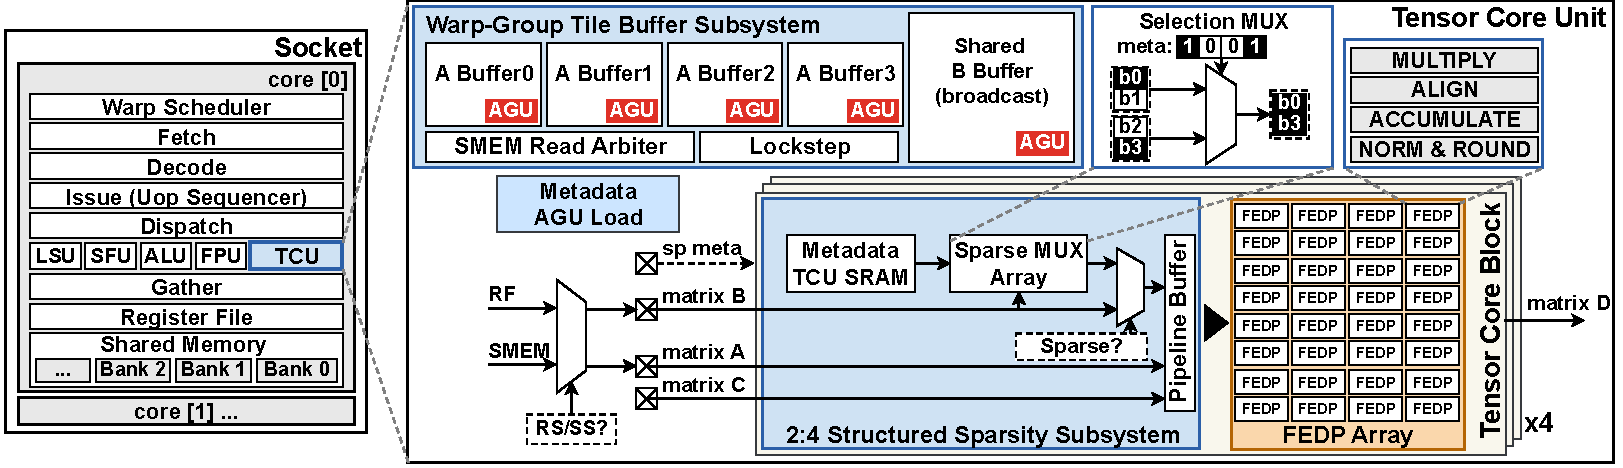
\includegraphics[width=\textwidth]{hpca2027-latex-template/fig/fourshadow_uarch_v3.pdf}
    \caption{FourShadow's complete datapath with Warp-Group and 2:4 Structured Sparsity subsystem extensions to the base Vortex GPGPU Tensor Core Unit.}
    \label{fig:figure_integration}
\end{figure*}

\subsection{Overview of FourShadow}
\label{sec:design_overview}

FourShadow adds two components to the base tensor core of Section~\ref{sec:bg_tcu}, the warp-group tensor core (Section~\ref{sec:design_wgmma}), which reads its operands from shared memory through the Warp-Group Tile Buffer Subsystem, and the sparse tensor core (Section~\ref{sec:design_sparse}), which adds 2:4 structured sparsity; Figure~\ref{fig:figure_integration} shows the complete datapath with both. Section~\ref{sec:design_pm} describes the programming model that selects among warp-level MMA, warp-group MMA and their sparse forms at compile time.

\subsection{Warp-group Tensor Core}\label{sec:design_wgmma}

\begin{figure}[t]
    \centering
    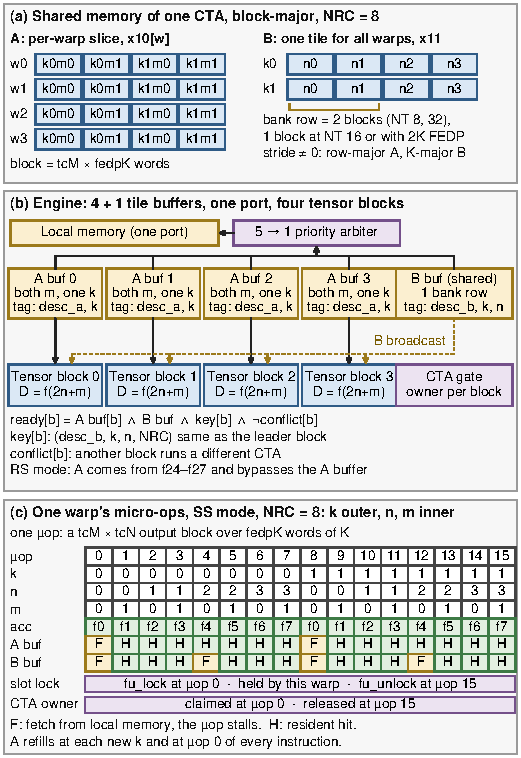
\includegraphics[width=\linewidth]{hpca2027-latex-template/fig/wgmma_operation.pdf}
    \caption{Warp-group MMA on FourShadow at an issue width of 4, SS mode, 8 or 32 threads per warp, standard FEDP. (a)~Block-major shared-memory layout of one CTA: each warp's slice of $A$ under its \texttt{x10} descriptor, one $B$ tile under \texttt{x11}. (b)~The engine: four $A$ buffers and one shared $B$ buffer behind one direct-access port, the tensor blocks and the CTA gate; $\mathit{ready}[b]$ combines the three consistency checks. (c)~The 16 micro-ops of one warp at $\mathit{NRC}{=}8$ with the accumulator of each, the $A$- and $B$-buffer fetches (F) and hits (H), and the span of the issue-slot lock and CTA ownership. In RS mode $A$ comes from \texttt{f24}--\texttt{f27} and bypasses the $A$ buffer; dense RS with the 2K-wide FEDP adds one setup micro-op.}
    \label{fig:wgmma_operation}
\end{figure}

\textbf{Warpgroup and tensor blocks.} The warp-group tensor core executes the warp-group MMA (WGMMA) instruction, with which the warps of a warpgroup compute one matrix product, each warp on its own tensor block. The core has one tensor block per issue slot, $\mathit{IW}$ blocks for an issue width of $\mathit{IW}$, and a warp runs on the block selected by its warp index modulo $\mathit{IW}$. Software forms the warpgroup: the kernel launches a cooperative thread array (CTA) of $\mathit{IW}$ warps, and warp $w$ of the CTA owns the $2\,\mathit{tcM}$ output rows that start at row $2w\,\mathit{tcM}$. All warps read the same $B$ tile, so a warpgroup extends the operation in the $M$ dimension only (Fig.~\ref{fig:wgmma_operation}(a): each warp supplies its own slice of $A$ and all warps read the same $B$ tile, so only the $M$ extent of the warp-group tile, $2\,\mathit{IW}\,\mathit{tcM}$, grows with $\mathit{IW}$). With $\mathit{NT}{=}32$ and $\mathit{IW}{=}4$, four $8{\times}4$ blocks compute a 64-row tile.

\textbf{Tile and micro-ops.} Each warp's sequencer expands its WGMMA instruction into micro-ops, and one micro-op computes one $\mathit{tcM}{\times}\mathit{tcN}$ block of the output over $\mathit{fedpK}$ words of $K$ ($\mathit{fedpK}{=}\mathit{tcK}$ for the standard FEDP). The per-warp tile is two blocks deep in $M$ and two in $K$, and the number of accumulator registers, $\mathit{NRC}\in\{8,16,32\}$, sets its extent in $N$:
\begin{equation}\label{eq:wg_tile}
\begin{aligned}
&\mathit{xtileN}_{\mathrm{wg}} = \tfrac{\mathit{NRC}\,\mathit{NT}}{2\,\mathit{tcM}},\;\;
m_{\mathrm{steps}} = 2,\\
&n_{\mathrm{steps}} = \tfrac{\mathit{xtileN}_{\mathrm{wg}}}{\mathit{tcN}} = \tfrac{\mathit{NRC}}{2},\;\;
k_{\mathrm{steps}} = \tfrac{2\,\mathit{tcK}}{\mathit{fedpK}}.
\end{aligned}
\end{equation}
$\mathit{NRC}{=}8$ is the accumulator count of the base tensor core. The micro-ops run with $k$ outermost, then $n$, then $m$ innermost, and micro-op $(m,n)$ accumulates into register \texttt{f}$(2n{+}m)$ (Fig.~\ref{fig:wgmma_operation}(c)). For $\mathit{NT}{=}32$, $\mathit{IW}{=}4$ and FP16 inputs, the warpgroup tile ($M{\times}N{\times}K$) is $64{\times}16{\times}16$ with 16 micro-ops per warp at $\mathit{NRC}{=}8$, and $64{\times}64{\times}16$ with 64 at $\mathit{NRC}{=}32$.

\textbf{Operands and descriptors.} Operand $B$ always comes from shared memory. Operand $A$ comes from shared memory in shared-memory/shared-memory (SS) mode and from four registers, \texttt{f24}--\texttt{f27}, in register/shared-memory (RS) mode. A shared-memory operand is named by a 32-bit descriptor: a 16-bit byte offset from the base of shared memory and a 16-bit row stride. A stride of zero selects the block-major layout, in which the tile is stored as the blocks that the micro-ops consume (Fig.~\ref{fig:wgmma_operation}(a)); a non-zero stride selects a row-major layout for $A$ and a K-major layout for $B$, from which the tile buffer gathers a block row by row. Software places the two descriptors in integer registers \texttt{x10} and \texttt{x11}, and each tensor block latches them at the first compute micro-op of the instruction. The accumulators occupy \texttt{f0} to \texttt{f}$(\mathit{NRC}{-}1)$, so $\mathit{NRC}{=}32$ fills the floating-point register file and is available in SS mode only; RS mode supports $\mathit{NRC}\le 16$. The kernel stages the tiles into shared memory with ordinary loads and stores or with DXA (Section~\ref{sec:bg_smem}), whose row-major output the non-zero-stride layout reads.

\textbf{Tile buffers and the shared-memory port.} Each tensor block has a private $A$ buffer that holds one $K$ stripe of its warp's tile, both $m$ blocks, and one $B$ buffer is shared by all tensor blocks: it holds the bank row that contains the $B$ block of the current $(k,n)$ and broadcasts it (Fig.~\ref{fig:wgmma_operation}(b)). The F and H rows of Fig.~\ref{fig:wgmma_operation}(c) give the fetch pattern: the $A$ buffer refills at every new $k$ and at the first compute micro-op of every instruction, because the kernel rewrites the tile in place under an unchanged descriptor, and one $B$ refill serves both $m$ micro-ops of all $\mathit{IW}$ blocks, eight tensor operations for $\mathit{IW}{=}4$, as long as the blocks request the same $(k,n)$. The simulated runs of Section~\ref{sec:eval_wgmma} realize this sharing: the shared-memory reads of an SS step amount to one $B$ tile per warpgroup, 1.00 at an issue width of four. The $\mathit{IW}{+}1$ buffers share, through a fixed-priority arbiter (the SMEM Read Arbiter of Figure~\ref{fig:figure_integration}), one port that reads a full bank row of $\mathit{NT}$ words per request. This port is the direct-access port of shared memory that DXA writes through, and it has priority over the load/store unit at every bank.

\textbf{Consistency without a barrier.} The warps of a warpgroup are not synchronized cycle by cycle: each warp's sequencer advances independently, and three checks, combined in the $\mathit{ready}[b]$ condition of Fig.~\ref{fig:wgmma_operation}(b), keep the shared state consistent. \emph{(i)~Issue-slot lock.} The first micro-op of an instruction locks its issue slot and the last releases it, so only that warp issues on the slot in between. \emph{(ii)~Single-CTA gate} (the Lockstep block of Figure~\ref{fig:figure_integration}). Each tensor block records the CTA of the instruction it executes from the first to the last compute micro-op, and a WGMMA micro-op waits while another block is inside an instruction of a different CTA. \emph{(iii)~$B$-key match.} The lowest-indexed active block sets the key of the shared $B$ buffer: the offset of the $B$ descriptor, $k$, $n$ and $\mathit{NRC}$. A block whose key differs stalls until the keys agree, and an idle block matches any key, so a CTA with fewer than $\mathit{IW}$ active warps runs unchanged. Each tensor block carries its results through its own result queue to commit.

\textbf{2K-wide FEDP.} The 2K-wide FEDP doubles the dot-product length from $\mathit{tcK}$ to $2\,\mathit{tcK}$ words for every input format, so one micro-op consumes both $K$ blocks of the tile and the dense $K$ steps go from two to one.

In SS mode both halves come from the tile buffers. In dense RS mode a compute micro-op needs two $A$ registers, and its second source field carries the upper half of $A$ in place of the $B$ descriptor; one setup micro-op therefore delivers the $B$ descriptor first, and the compute micro-op for block $m$ reads the lower half of $A$ from \texttt{f}$(24{+}2m)$ and the upper half from \texttt{f}$(25{+}2m)$. The upper half of both operands is zero for WMMA and for sparse WGMMA, which takes one $K$ step with or without the 2K-wide FEDP, so both instructions execute unchanged. We stop at 2K: a wider FEDP makes every unit more expensive and adds fanout across the datapath, and its upper part is idle for every WMMA and sparse instruction.

\textbf{Explored alternatives.} Section~\ref{sec:eval_wgmma} also evaluates two variants of this design.
% TODO(ispass): not in pinned branch d6426cca1 (FEDP latency there does not depend on FEDP2K); data from an earlier commit -- coauthors confirm the commit behind the data.
The first deepens the FEDP pipeline from four to eight cycles, to absorb the longer multiply and accumulate stages of a 2K-wide unit; its cost is a longer latency for every WMMA and WGMMA micro-op.
% TODO(ispass): not in pinned branch d6426cca1 (the metadata SRAM there has only sparse and MX namespaces); data from an earlier commit (results file added in 814951568) -- coauthors confirm the commit behind the data.
The second holds the descriptors in the per-warp TCU SRAM that stores the sparse metadata (Section~\ref{sec:design_sparse}) in place of \texttt{x10} and \texttt{x11}: the warp writes its descriptors to shared memory and loads them with the metadata-load instruction. This relieves the register file, and its cost is a shared-memory store, a CTA barrier and a load through the load/store unit before the first micro-op.

\subsection{Sparse Tensor Core}\label{sec:design_sparse}

\textbf{2:4 Structured Sparsity.} The sparse tensor core executes WMMA and WGMMA on a matrix $A$ pruned with 2:4 structured sparsity: every group of four consecutive elements along $K$ in a row of $A$ keeps two. $A$ is stored compressed, as its kept elements, with metadata whose bits mark the kept positions of each row; $B$ stays dense.

\textbf{Microarchitecture.} Figure~\ref{fig:figure_integration} draws the sparse tensor core as the 2:4 Structured Sparsity Subsystem, between the operands and the FEDP arrays. The Metadata AGU Load block brings the metadata into the Metadata TCU SRAM. The Sparse MUX Array receives matrix $B$ and the metadata of the current micro-op and selects, for each row of $A$, the two elements of every group of four $B$ candidates that match the kept positions of that row (one of every two for 32-bit inputs); in the Selection MUX inset, metadata 1001 selects $b_0$ and $b_3$. The array has one selector per FEDP unit, because the rows of $A$ keep different positions of the same $B$ candidates. A multiplexer passes the selected $B$, or the unmodified $B$ of a dense instruction, to the Pipeline Buffer. Compressed $A$ reaches the FEDP arrays as stored, without inserted zeros, so an FEDP unit computes as many products as in a dense micro-op but covers twice the positions of $K$, which halves the $K$ steps of a tile.

\textbf{Sparse Metadata Flow.} Before sparse execution the kernel calls \texttt{load\_sp\_metadata}, which emits one warp-level instruction, \texttt{TCU\_LD}: each lane contributes one 32-bit metadata word, and a warp-level address generation unit (AGU) issues the load as an ordinary load/store request. The request is routed by its address like any other load, to global or to shared memory; our sparse kernels keep the metadata in global memory. The returned words are written to the metadata SRAM of every tensor block, indexed by warp, and a micro-op reads the part selected by its $m$ and $k$ steps, so any tensor block can run that warp's sparse micro-ops. In the RTL the scoreboard orders the two operations: the decoder marks the metadata load as the writer of a reserved per-warp scoreboard bit and every sparse MMA as a reader of it, and the bit is released by the writeback of the load, which the AGU raises in the cycle it writes the SRAM, so a sparse MMA issues only after its metadata is written, without a software-visible fence.

\textbf{Asymmetric vs.\ Symmetric Configurations.} The halved $K$ steps halve the micro-ops of a sparse WMMA only in the asymmetric configurations of Section~\ref{sec:bg_tcu} ($\mathit{NT}{\in}\{2,8,32\}$), a consequence of the four registers a micro-op names (Section~\ref{sec:design_pm}). A sparse micro-op needs twice the $B$ of a dense one (the red ``$\times$2 col candidates'' of Figure~\ref{fig:figure_register_mapping}). In the asymmetric case, panel~(a) with $\mathit{NT}{=}8$, a dense block of $B$ occupies half a register, so the doubled block fits in the one $B$ register that the micro-op already reads (red \texttt{reg0}). In the red annotations, $\mathit{xtileK}$ halves from 8 to 4 and $k_{\mathrm{steps}}$ from 4 to 2, so the micro-ops halve from 32 to 16 with every FEDP unit active.

In the symmetric case, panel~(b) with $\mathit{NT}{=}4$, a dense block of $B$, $\mathit{tcK}{\times}\mathit{tcN} = 2{\times}2$ words, already fills a register, and the doubled block would need a second $B$ register, which a micro-op cannot name: its four register fields hold $A$, $B$, $C$ and $D$. The symmetric configurations therefore halve $\mathit{tcN}$ from 2 to 1, which doubles $n_{\mathrm{steps}}$ from 2 to 4 while $k_{\mathrm{steps}}$ halves from 2 to 1 (red annotations of panel~(b)): a thread mask activates half the FEDP units in each micro-op, and the micro-op count stays at 16.

\subsection{Programming Model}
\begin{figure}
    \centering
    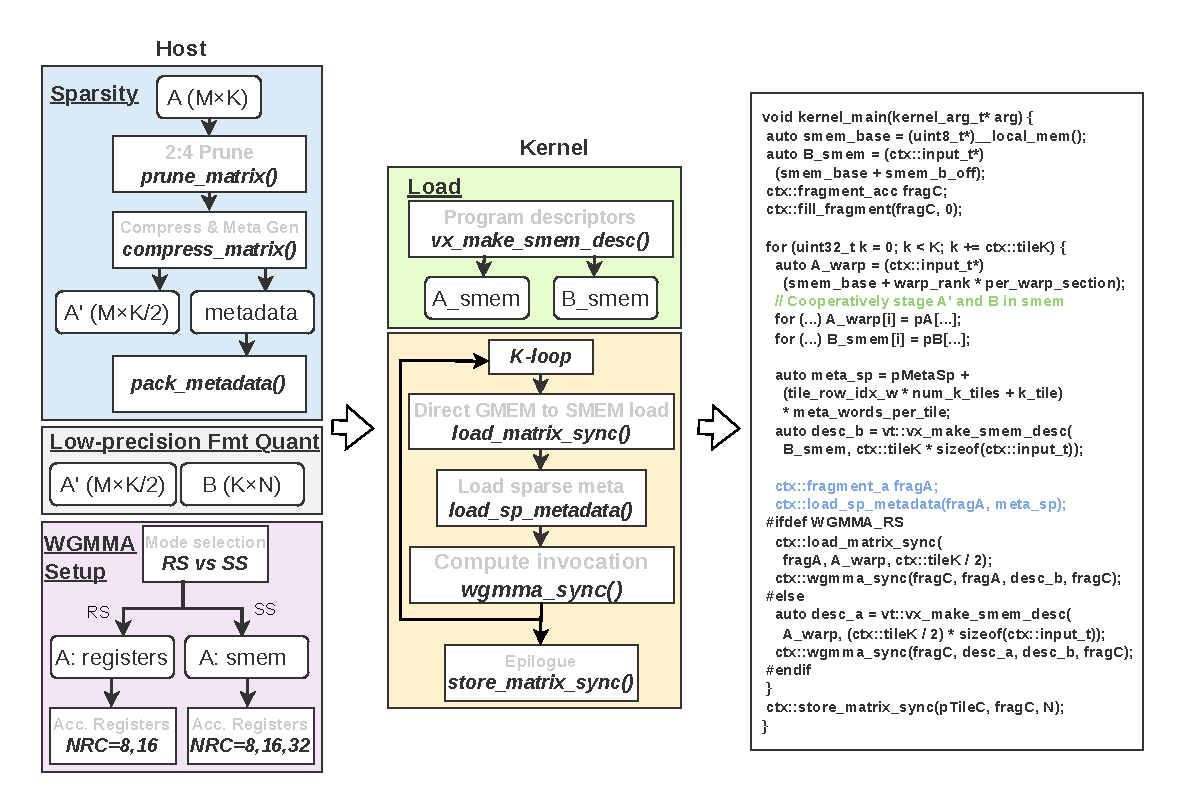
\includegraphics[width=\linewidth,trim=18 12 19 16,clip]{hpca2027-latex-template/fig/sw_integrationv4.pdf}
    \caption{FourShadow Programming Model}
    \label{fig:sw_integrationv4}
\end{figure}
\label{sec:sw_integrationv4}\label{sec:design_pm}

FourShadow exposes WMMA, WGMMA, and 2:4 structured sparsity as composable primitives selected almost entirely at compile time. Input/output format (\texttt{ITYPE}/\texttt{OTYPE}), NRC, and RS-versus-SS mode (Section~\ref{sec:design_wgmma}) are all template parameters on \texttt{wgmma\_config\_t} and \texttt{wgmma\_context} (Figure~\ref{fig:sw_integrationv4}), so the same kernel source compiles down to dense WMMA, dense WGMMA, or sparse WGMMA execution depending on how it is instantiated.

\begin{comment}
\begin{table}[t]
\centering
\caption{RISC-V encoding of the tensor-core instructions (R-type, opcode 0x0B, funct7 0x02).}
\label{tab:isa}
\footnotesize
\setlength{\tabcolsep}{4pt}
\begin{tabular}{@{}l l l l@{}}
\toprule
 & \textbf{WMMA} & \textbf{WGMMA} & \textbf{\texttt{TCU\_LD}} \\
\midrule
funct3 & 0 & 1 & 2 \\
rd & output format & output format & metadata slot \\
rs1 & input format & input format & address register \\
rs2 & sparse & sparse, $\mathit{NRC}$, SS/RS & input format \\
\midrule
$C/D$ & \texttt{f0}--\texttt{f7} & \texttt{f0}--\texttt{f}$(\mathit{NRC}{-}1)$ & -- \\
$A$ & \texttt{f10}--\texttt{f17} & \texttt{x10} or \texttt{f24}--\texttt{f27} & -- \\
$B$ & \texttt{f24}--\texttt{f31} & \texttt{x11} & -- \\
\bottomrule
\end{tabular}
\end{table}
\end{comment}

% ISA table removed; its text commented out with it.
% \textbf{Instruction encoding.} The three tensor-core instructions are 32-bit RISC-V R-type instructions in the CUSTOM-0 opcode space (0x0B) with funct7 0x02, and funct3 selects the instruction (Table~\ref{tab:isa}). In WMMA and WGMMA the rd, rs1 and rs2 fields hold immediates, not register numbers: the output format, the input format and flags that mark a sparse instruction and, for WGMMA, select $\mathit{NRC}$ and SS or RS mode. The operands sit in fixed registers (last three rows); for WGMMA, \texttt{x10} and \texttt{x11} hold the shared-memory descriptors of Section~\ref{sec:design_wgmma}. The sequencer expands an instruction into micro-ops in the loop order of Figs.~\ref{fig:tiling_equations} and~\ref{fig:wgmma_tiling_equations}, and each micro-op names four registers: $A$ or its descriptor in rs1, $B$ or its descriptor in rs2, and the accumulator in rs3 as $C$ and in rd as $D$. \texttt{TCU\_LD} reads its one register operand, the metadata address, from rs1 (Section~\ref{sec:design_sparse}).

\textbf{Metadata packing.} On the host, \texttt{pack\_metadata\_wg} repacks the 2:4 mask produced by pruning/compression into the per-thread SRAM bank layout that the \texttt{TCU\_LD} AGU and the metadata SRAM expect (Section~\ref{sec:design_sparse}); the layout is dimensioned against the \emph{WMMA}-config per-warp depth, since that shared hardware is sized for WMMA.

\textbf{Operand and metadata delivery.} In the kernel, \texttt{load\_sp\_metadata} loads the packed mask in both RS and SS mode (Section~\ref{sec:design_sparse}), and $A$ reaches the instruction as Section~\ref{sec:design_wgmma} describes, through \texttt{load\_matrix\_sync} in RS mode and through a descriptor built by \texttt{vx\_make\_smem\_desc} in SS mode; both modes call the same \texttt{wgmma\_sync} entry point.

\textbf{Tile Stride.} Each warp's private $A$ section is padded to the shared-memory bank-row width ($\mathit{NT}\times\mathrm{XLEN}/8$ bytes) so warp $w{+}1$'s stripe always starts on a fresh bank row. Without this, the $A$ buffer's single-row fetch can walk into the previous warp's region.
\section{Methodology}
\label{sec:methodology}

FourShadow is implemented in Vortex~\cite{vortex}, the open-source RISC-V GPU, and its performance is measured there: in processor cycles on SimX, the Vortex cycle-level simulator, and end to end on an FPGA. FourShadow is compared with two NVIDIA GPUs, an RTX 5080 and an H100, for the reasons given in Section~\ref{sec:intro}. Because the NVIDIA GPUs run different toolkits and FourShadow counts simulated cycles, the platforms are compared only by ratios and trends, never by absolute cycles.

\subsection{Hardware Configuration}\label{sec:method_hw}

Table~\ref{tab:config} lists the configuration of each platform; every run uses one FourShadow core and one SM of each GPU. FourShadow's entries are Vortex build options, with the tensor core, warp-group MMA and DXA enabled; only the accumulator count $\mathit{NRC}$ is a kernel parameter; parentheses name the part of Section~\ref{sec:eval} that sweeps a value, and bold marks the default (an issue width cannot exceed NW). We name a FourShadow configuration by its issue width (IW) and its number of warps per core (NW): (IW-1, NW-4) issues from one warp per cycle on a core of four warps; every part that runs four warps per core states it. The configuration matched to the H100 is (IW-4, NW-4) at 32 threads per warp. The H100 has no $\mathit{NRC}$; each $\mathit{NRC}$ is paired with the \texttt{wgmma.m64nNk16} of equal warp-group tile, $N{=}\mathit{NRC}\,\mathit{NT}/(2\,\mathit{tcM}){=}2\,\mathit{NRC}$ (Eq.~\ref{eq:wg_tile}), whose 128 threads each hold $N/2{=}\mathit{NRC}$ FP32 accumulators~\cite{nvidia2026ptxisa}.

\begin{table}[h]
\centering
\caption{Microarchitecture Configuration Comparison between FourShadow and NVIDIA GPUs}
\label{tab:config}
\footnotesize
\setlength{\tabcolsep}{2pt}
\renewcommand{\arraystretch}{0.95}
\begin{tabular}{@{}l l l l@{}}
\toprule
 & \textbf{FourShadow} & \textbf{RTX 5080} & \textbf{H100 SXM} \\
\midrule
Threads/warp (NT) & 4, 8, 16, 32 (\ref{sec:eval_threads}) & 32 & 32 \\
Warps/core (NW) & 4, 16 & 4 per CTA & 4 per CTA \\
Issue width (IW) & 1, 2, 4, 8 (\ref{sec:eval_iw}) & -- & 4 (warpgroup) \\
Accum.\ regs.\ ($\mathit{NRC}$) & 8, 16, 32 (\ref{sec:eval_nrc}) & -- & -- \\
FEDP width & $K$, $2K$ (\ref{sec:eval_fedp2k}) & not visible & not visible \\
Warp-level MMA & TCU, dense, 2:4 & \texttt{mma(.sp)} & \texttt{mma(.sp)} \\
Warp-group MMA & WGMMA, RS, SS & -- & \texttt{wgmma(.sp)} \\
\midrule
Cycles & simulated & \texttt{clock64} & \texttt{clock64} \\
Tech. Node. & ASAP7 & TSMC 4NP & TSMC 4N \\
Clock Freq. & 1.0 GHz & 2.295 GHz & 1.59 GHz \\
Toolchain & \makecell[l]{VOLT~\cite{10.1145/3771775.3786275},\\\texttt{Vortex 3.0}} & \makecell[l]{CUDA 13.0,\\\texttt{sm\_120a}} & \makecell[l]{CUDA 12.4.131,\\\texttt{sm\_90a}} \\


\bottomrule
\end{tabular}
\end{table}

\subsection{Software Configuration}\label{sec:method_sw}

The design-space sweeps run $128\times128\times K$ SGEMM kernels, where $K\in\{128,256,512,1024\}$, change one architectural parameter while holding the rest of the configuration fixed, and compute speedups from total kernel cycles against the baseline configuration each part names in the (IW-N, NW-M) form; the figures show these kernels. \phantomsection\label{sec:large_method}We repeat these sweeps at $256{\times}256{\times}K$ and $512{\times}512{\times}K$ with $K\in\{128,256,512,768,1024,1536\}$, and \phantomsection\label{sec:skinny_method}on skinny GEMMs, tall ($128{\times}n{\times}K$) and wide ($n{\times}128{\times}K$), with $n$ of 16 to 64 and $K$ up to 1536.
% Source (skinny): 00_doc/vortex-wgdxa2k/results/SKINNY.md sections 1 and 5 (S = 128 family; views t16/t32/t64, w16/w64; K 128-1536; items F1-F11 = every 128x128 sweep but the descriptor load), results/skinny.json.
The comparisons with the NVIDIA GPUs run instruction-level kernels and count cycles over an in-kernel region. Warp-level MMA is compared at (IW-1, NW-4) with 8 or 32 threads per warp, because there the FP16 sparse speedups of FourShadow and the RTX 5080, over the 17 shapes measured on both, differ by a median of 9.0\% at 8 threads and 6.2\% at 32 threads, less than at issue widths of 2 and 4.

\section{Evaluation}\label{sec:eval}

\subsection{Scaling Across the SIMT Hierarchy}\label{sec:eval_hierarchy}

The last parts of Sections~\ref{sec:eval_threads} and~\ref{sec:eval_iw} answer Q2 (Section~\ref{sec:intro}) at the design points around NVIDIA's.

\subsubsection{Threads/Warp}\label{sec:eval_threads}
Fig.~\ref{fig:threads_sweep}(a) compares TCU SGEMM with scalar FP32 execution
at the same thread count. Packing more low-precision elements raises
speedup from 3.55--6.44$\times$ for TF32 to 9.53--27.46$\times$ for FP8.
Most notably, we find that the 16-thread configuration is consistently the strongest and reaches
27.46$\times$, while increasing to 32 threads (the established default warp-size in all modern GPU architectures) does not improve performance
further. This shows that Tensor Core scaling is non-monotonic with warp width
and depends significantly on tile geometry and pipeline utilization.

Warp-group MMA keeps this advantage, as the Block equations of Fig.~\ref{fig:tiling_equations} show. Eqs.~(\ref{eq:block_cap})--(\ref{eq:block_tc}) arrange the $\mathit{block\_cap}{=}\mathit{NT}$ FEDP units of a micro-op as a near-square $\mathit{tcM}{\times}\mathit{tcN}$ grid, and each lane's dot product is $\mathit{tcK}{=}\mathit{block\_cap}/\max(\mathit{tcM},\mathit{tcN})$ words: the block is $4{\times}2{\times}2$, $4{\times}4{\times}4$ and $8{\times}4{\times}4$ at 8, 16 and 32 threads, or 4, 8 and 8 FP16 multiply-accumulates (MACs) per lane and micro-op. A warp issues $2\,\mathit{NRC}$ micro-ops per dense step at every $\mathit{NT}$ (Fig.~\ref{fig:wgmma_operation}(c)), each at a fixed cost, plus about one cycle per 64-byte operand line. A lane's work thus doubles from 8 to 16 threads but not from 16 to 32, where only $\mathit{tcM}$ doubles, and with it $A$: 16 to 32 shared-memory lines per SS step ($\mathit{IW}{=}4$, $\mathit{NRC}{=}32$). In MACs per cycle over the warpgroup's $\mathit{IW}{\times}\mathit{NT}$ threads, from back-to-back FP16 warp-group MMAs at (IW-4, NW-4), 16 threads is 11--19\% ahead of 32 in SS mode (3.48 against 3.14 at $\mathit{NRC}{=}32$, Fig.~\ref{fig:q2_nt_iw}(a)) and level in RS mode.

\answerbox{Answer \#1 for Q2}{Per-lane warp-group MMA throughput peaks at 16 threads per warp, because a lane's dot product doubles from 8 to 16 threads but not from 16 to 32; NVIDIA's 32-thread point sits on this plateau (level in RS mode, 11--19\% behind in SS mode).}

\begin{figure}
    \centering
    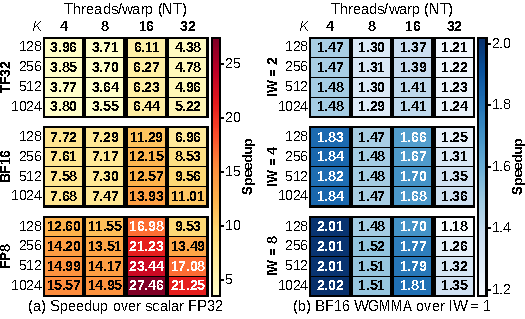
\includegraphics[width=\columnwidth]
    {hpca2027-latex-template/fig/eval_nt_iw_heatmaps.pdf}
    \caption{(a)~SGEMM speedup over scalar FP32 execution across
    threads/warp and input precisions. (b)~BF16 WGMMA speedup over an
    issue width of one across threads/warp and issue-width configurations,
    four warps per core (eight at an issue width of 8, as IW${\le}$NW).}
    \label{fig:threads_sweep}
    \label{fig:iw_sweep}
\end{figure}

\begin{figure}[t]
    \centering
    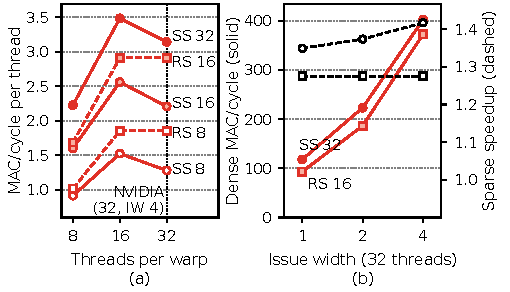
\includegraphics[width=\linewidth]
    {hpca2027-latex-template/fig/paper_q2_nt_iw.pdf}
    \caption{Warp-group MMA throughput on FourShadow around NVIDIA's design
    point, four warps per core, lines labelled by mode and $\mathit{NRC}$: (a)~against
    threads per warp at (IW-4, NW-4); (b)~dense throughput and sparse speedup
    against the issue width at 32 threads per warp.}
    \label{fig:q2_nt_iw}
\end{figure}

% float placed early: renders at the top of the right column beside the roofline subsection (sec:eval_roofline)
\begin{figure}
    \centering
    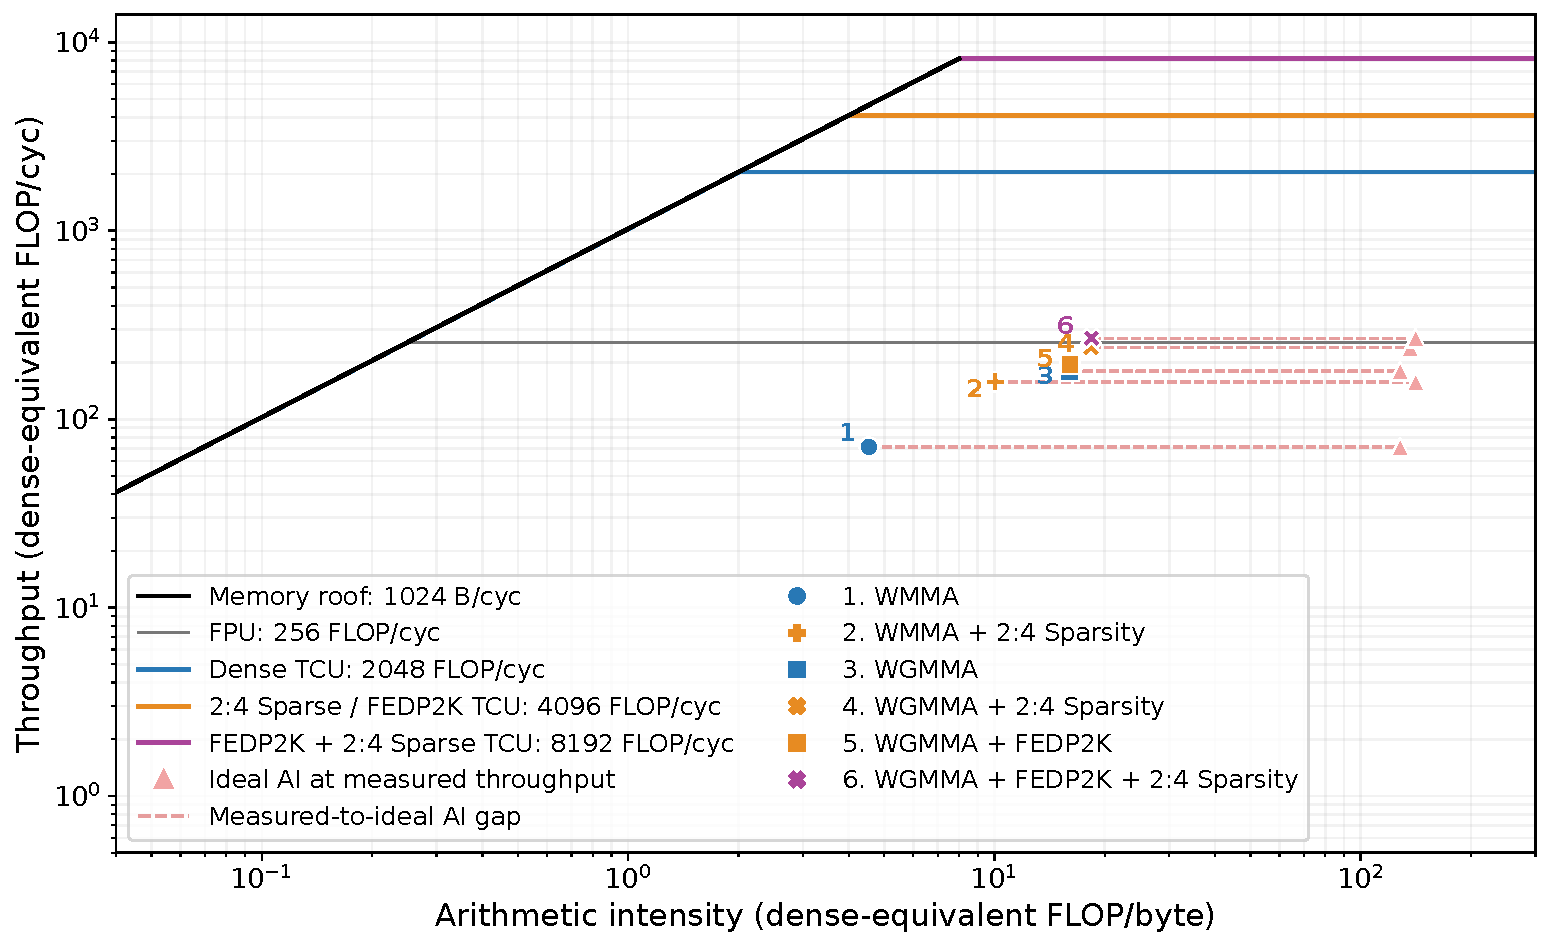
\includegraphics[width=\linewidth]
    {hpca2027-latex-template/fig/roofline_512.pdf}
    \caption{Roofline analysis of $512^3$ SGEMM on FourShadow analyzing WMMA, WGMMA, 2:4 Structuted Sparsity and FEDP2K extensions.}
    \label{fig:roofline}
\end{figure}

\subsubsection{Warps/Warpgroup (Issue Width)}\label{sec:eval_iw}
Fig.~\ref{fig:iw_sweep}(b) normalizes each configuration against an issue
width of one. An issue width of two provides 1.21--1.48$\times$ speedup,
while four reaches up to 1.84$\times$. Increasing to eight only peaks at 2.02$\times$, with the 8- and 16-thread designs largely saturating after
four. The returns diminish because instruction issue, not the tensor core or shared memory, bounds the kernel. In the dense warp-group GEMM loop at (IW-4, NW-4), 8 threads per warp and $\mathit{NRC}{=}8$, the warp-group MMA is 2.1--2.5\% of a $K$ step, and the rest stages $A$ and $B$ into shared memory on the integer and load/store units. With four warps per core, the kernel issues 0.42--0.44 instructions per cycle at every issue width and uses 1.5--1.7\% of the shared-memory bank bandwidth, so a wider issue gains only the instructions saved by staging $B$ once for a larger warpgroup. Growing the warps with the issue width, to (IW-2, NW-8), (IW-4, NW-16) and (IW-8, NW-32), speeds up a $K$ step over (IW-1, NW-4) by 2.4--2.5$\times$, 3.2--3.5$\times$ and 3.6--3.9$\times$ rather than 2, 4 and 8$\times$: from (IW-4, NW-16) on, the core schedules a warp in 93--99\% of cycles, because its front end fetches one warp instruction per cycle whatever the issue width. The warp-group MMA escapes this bound because each instruction expands into $2\,\mathit{NRC}$ micro-ops that keep its warp's tensor block busy.
% Sources: 00_doc/vortex-wgdxa2k/results/SMEM_BW_IW.md (staging IPC, banks), IW_NW_SWEEP.md sections 2 and 4 (NW-4 IPC 0.416-0.437, bank use 0.015-0.017) + iw_nw_sweep.json (diagonal, sched. busy); fetch: SimX core.cpp:330-358.
% TODO(ispass): fig:iw_sweep(b) -- the printed IW-8 row (1.18--2.02x over IW 1) is not reproduced; the final SimX (IW-8, NW-8) cell gives 2.80--3.20x per K step (IW_NW_SWEEP.md section 3).

At the instruction level, the warp-group MMA of FourShadow scales nearly linearly with the issue width. Fig.~\ref{fig:q2_nt_iw}(b) streams back-to-back warp-group MMAs at 32 threads per warp, four warps per core and issue widths of 1, 2 and 4, a narrower range than the whole-kernel sweep of Fig.~\ref{fig:iw_sweep}(b), which extends to 8. Each doubling of the issue width raises throughput by $\times$2.00 and again by $\times$2.00 in RS mode at $\mathit{NRC}{=}16$, and by $\times$1.89 and then $\times$1.80 in SS mode at $\mathit{NRC}{=}32$. As the issue width grows, the sparse per-$K$ speedup stays at 1.275$\times$ in RS mode and rises from 1.349$\times$ to 1.417$\times$ in SS mode. Sparsity shortens the fixed micro-op part of a step, from 72 to 53 cycles in RS mode at $\mathit{NRC}{=}16$. The issue-width results are measured on FourShadow alone; a commercial GPU fixes its warpgroup at four warps. \phantomsection\label{sec:skinny_iw}The instruction-issue bound holds for skinny GEMMs: (IW-8, NW-32) speeds up a $K$ step over (IW-1, NW-4) by 3.84--3.91$\times$ on wide shapes at 8 threads per warp, and by 2.88--3.74$\times$ on tall shapes with $N{=}16$, where fewer warps have work.
% Source (skinny): SKINNY.md section 5.4 row 16 and skinny.json families.128 claim F3.diag8.avail (w64 = 64x128xK, NT 8 RS/SS only: the 32-thread IW-8 CTA (M 128) cannot tile M = 64; t16 = 128x16xK, NT 8/32 RS/SS); idle warps at t16: SKINNY.md 5.3 finding 2.

\answerbox{Answer \#2 for Q2}{A wider warpgroup scales the warp-group MMA but not the kernel around it: the core fetches one warp instruction per cycle, so the kernel's other instructions issue at most about one per cycle, while each warp-group MMA expands into $2\,\mathit{NRC}$ micro-ops that keep its tensor block busy; with the warps grown to match, an issue width of 8 speeds up a $K$ step of the GEMM by 3.6--3.9$\times$, not 8$\times$.}


\subsubsection{Roofline Model Performance Analysis}\label{sec:eval_roofline}
Fig.~\ref{fig:roofline} evaluates $512^3$ SGEMM on SimX with
FP16 inputs and FP32 accumulation, on a Vortex configuration closely modeling an equivalent NVIDIA H100 SM (32 threads/warp, 64 resident warps/core, issue width 4, four DXA workers, 64\,KB shared memory and memory-BW roof of 1024\,B/cyc).
Both throughput and arithmetic intensity use the dense-equivalent
operation count $2MNK$, for 2:4 sparse execution as well. The ideal arithmetic intensity counts one read of each input and one
write of the output, including compressed $A$ and padded metadata for
sparse execution. Deep-buffered WGMMA with DXA increases arithmetic intensity from WMMA's
4.54 to 16.04 FLOP/byte and throughput from 71.22 to 179.17 FLOP/cyc,
a 2.52$\times$ speedup. With 2:4 sparsity, WMMA reaches
157.72 FLOP/cyc and WGMMA reaches 239.66 FLOP/cyc.
FEDP2K alone changes dense WGMMA throughput only slightly, to
180.48 FLOP/cyc, while combining it with sparsity reaches
268.85 FLOP/cyc, 1.50$\times$ dense WGMMA and 3.77$\times$ dense WMMA. This indicates that these modern Tensor Core extensions (2:4 Stuctured Sparsity, WGMMA, FEDP2K) are helping move fairly memory-bound kernels into the compute bound region. WGMMA
specifically seems to be improving arithmetic intensity significantly from
it’s larger operating tiles and shared-memory reuse, making it
particularly suitable for modern ML systems inference workloads that are heavily memory-bound at small batch sizes.

\subsection{Warp-Group Tensor Core Design Space Exploration}\label{sec:eval_wgmma}

The first three parts explore FourShadow's warp-group design space; the fourth answers Q1 (Section~\ref{sec:intro}) for warp-group MMA against an H100, and Section~\ref{sec:eval_sparse} continues Q1 for sparsity.

\subsubsection{Number of Accumulator Registers (NRC) Scaling}\label{sec:eval_nrc}
\begin{figure}[t]
    \centering
    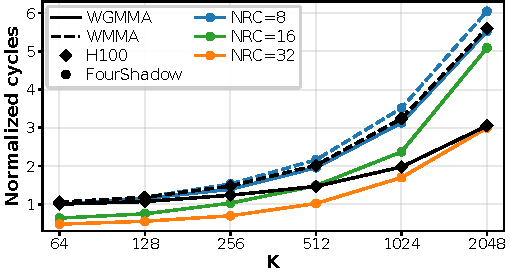
\includegraphics[width=\linewidth,trim=0 4 0 0,clip]
    {hpca2027-latex-template/fig/nrc_h100_scaling.pdf}
    \caption{FP16 WMMA and WGMMA cycles as $K$ grows on FourShadow and an
    H100, each normalized to the platform's WGMMA at $K{=}64$
    ($\mathit{NRC}{=}8$ on FourShadow).}
    \label{fig:nrc_h100}
\end{figure}

Fig.~\ref{fig:nrc_h100} compares how FP16 WMMA and WGMMA scale with $K$ on FourShadow and an H100, each platform normalized to its WGMMA cycles at $K{=}64$. It suggests that limited accumulator capacity is one reason WMMA attains only about 63\% of peak throughput on Hopper, against over 95\% for WGMMA~\cite{luo2025dissectingnvidiahopperarchitecture}. With $\mathit{NRC}{=}8$, the accumulator count of WMMA, FourShadow's normalized cycles grow from 1.00$\times$ to 5.52$\times$ as $K$ grows to 2048, close to the H100's WMMA curve; with $\mathit{NRC}{=}32$ they reach only 3.00$\times$, nearly the H100 WGMMA's 3.05$\times$ ($\mathit{NRC}{=}16$ reaches 5.09$\times$). Hopper's WGMMA performance gains over WMMA thus appear to primarily come from a larger effective accumulator tile size rather than just direct SMEM load.
\subsubsection{K vs.\ 2K-Wide FEDP}\label{sec:eval_fedp2k}
% TODO(ispass): fig:fedp2k_sweep -- FEDP bars not from the final runs; NRC-16 K-wide lat-4 bars differ from fig:nrc_h100
Fig.~\ref{fig:fedp2k_sweep} shows that the 2K-wide FEDP is able to reduce instruction count by 31--33\% and execution cycles by 28--30\% in both
operand-staging modes. Our evaluations also show that increasing FEDP pipeline latency from four to eight
cycles adds at most 3.1\% overhead. Halving the number of $K$-dimension
micro-ops therefore considerably outweighs the deeper pipeline and extra descriptor-setup micro-op cost.
% TODO(ispass): the next sentence moved here from the design section (a measurement); its source run is not identified in the pinned branch d6426cca1 -- coauthors confirm.
The setup micro-op that dense RS mode adds with the 2K-wide FEDP increases the end-to-end cycle count by under 1\%.
\begin{figure}
    \centering
    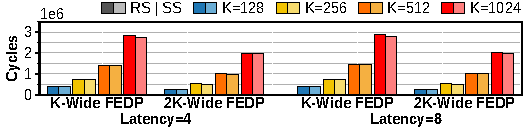
\includegraphics[width=\linewidth]
    {hpca2027-latex-template/fig/fedp2k_cycles_short.pdf}
    \caption{WGMMA execution cycles with $K$-wide and $2K$-wide FEDP
    units at four- and eight-cycle pipeline latencies.}
    \label{fig:fedp2k_sweep}
\end{figure}

% Descriptor-load study, removed for length; restore by uncommenting.
% \subsubsection{TCU SRAM vs.\ Register File WGMMA Descriptor Load}\label{sec:eval_desc}
% Moving the WGMMA descriptors into TCU SRAM increases cycles by
% 1.2--6.5\% relative to register-file delivery. The penalty is largest for short SS kernels
% and decreases as more computation amortizes descriptor setup. Relieving
% the pressure of two register operands does not offset the added
% shared-memory store, synchronization, and AGU traffic. Small control
% metadata should therefore remain in the register file unless those
% registers enable a larger accumulator configuration or there is extreme register pressure.

\begin{figure}[t]
    \centering
    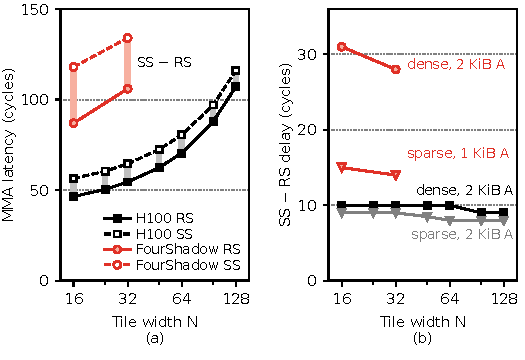
\includegraphics[width=\columnwidth,trim=0 6 1 0,clip]
    {hpca2027-latex-template/fig/delay_a.pdf}
    \caption{Delay for reading $A$ from shared memory (SS $-$ RS) in a warp-group
    MMA, FP16, on an H100 and FourShadow: (a)~latency against the tile width $N$;
    (b)~the delay, dense and sparse, labelled with the bytes of $A$.}
    \label{fig:delay_a}
\end{figure}

\begin{figure}[t]
    \centering
    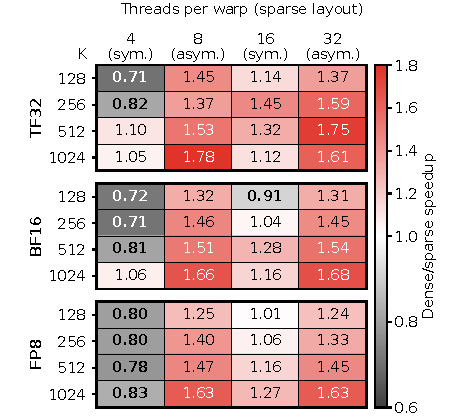
\includegraphics[width=0.9\linewidth]
    {hpca2027-latex-template/fig/sparse_sym_asym_iw1_nw4.pdf}
    \caption{Dense-over-sparse speedup of a $128{\times}128{\times}K$ GEMM
    with warp-level MMA at (IW-1, NW-4), from total kernel cycles on SimX.
    Each cell prints the speedup; cells below 1 (sparse slower than dense)
    are grey, cells above 1 red.}
    \label{fig:sparse_sym_sweep}
\end{figure}

\subsubsection{Reading \texorpdfstring{$A$}{A} from Shared Memory Delays Every Warp-Group MMA}\label{sec:eval_delay_a}
% TODO(ispass): the FourShadow delay values come from SimX, which fetches the whole A tile in 64-B lines; sec:design_wgmma describes the RTL A buffer (one K stripe, one bank row per request). See 00_doc/vortex-wgdxa2k/results/DELAY_A.md.
In RS mode the compute micro-ops read $A$ from registers \texttt{f24}--\texttt{f27}, and only $B$ crosses the shared-memory port. In SS mode each tensor block must fill its $A$ buffer through that port, which all $\mathit{IW}{+}1$ tile buffers share (Section~\ref{sec:design_wgmma}), so its first multiplication waits for those reads. Fig.~\ref{fig:delay_a} times each warp-group MMA after the previous one completes. On FourShadow at (IW-4, NW-4) and 32 threads per warp this wait adds 28--31 cycles to a dense warp-group MMA (bars in Fig.~\ref{fig:delay_a}(a)). It does not grow with $N$: $A$ is the $64{\times}16$ tile of every instruction, while $N$ widens only $B$ and the micro-ops, which both modes pay. It follows the bytes of $A$: the compressed 1\,KiB sparse $A$ pays 14--15 cycles (Fig.~\ref{fig:delay_a}(b)). It recurs on every instruction, because the $A$ buffer refills at each instruction's first compute micro-op (the F cells of Fig.~\ref{fig:wgmma_operation}(c)): a descriptor names an address, and the kernel may rewrite the tile under it. One warpgroup of the H100 shows all three signatures: dense SS mode completes 9.0--10.0 cycles after RS mode from $N{=}16$ to 128, sparse pays alike (8.0--9.0) because it also reads 2\,KiB of $A$, and the delay stays at 10.25 cycles when every instruction reads the same $A$. The H100's warp-group MMA thus behaves as one that stages $A$ from shared memory before its first multiplication and keeps no copy between instructions, as FourShadow does.

\answerbox{Answer \#1 for Q1}{A warp-group MMA in SS mode waits for $A$ before its first multiplication, a fixed delay per instruction that does not grow with the tile width; the H100 and FourShadow keep no operand between instructions, so every instruction pays the delay again.}

\subsection{Sparse Tensor Core Design Space Exploration}\label{sec:eval_sparse}

This subsection continues Q1 with the internal mechanisms behind tensor-core sparsity (Section~\ref{sec:intro}). The first part explores the symmetric and asymmetric layouts of warp-level MMA on FourShadow. The next two give the answers by comparing FourShadow with NVIDIA GPUs: warp-level MMA with 2:4 sparsity with an RTX 5080 and an H100, and warp-group MMA with an H100 (Sections~\ref{sec:eval_sparse_halves} and~\ref{sec:eval_sparse_wg}, configuration in Section~\ref{sec:methodology}).

\subsubsection{Symmetric vs.\ Asymmetric Sparse Configurations}\label{sec:eval_sparse_sym}
Sparsity speeds up the asymmetric layouts in every cell of
Fig.~\ref{fig:sparse_sym_sweep} and the symmetric layouts less. The 8- and
32-thread cells span 1.24--1.78$\times$, with the maximum for TF32 at
$K{=}1024$ and 8 threads, and both symmetric cells sit below both
asymmetric cells in 11 of 12 rows (the exception: TF32 at $K{=}256$,
1.45$\times$ at 16 threads against 1.37$\times$ at 8).
\phantomsection\label{sec:large_sym}The ordering holds at $256{\times}256{\times}K$ and $512{\times}512{\times}K$: the asymmetric cells span 1.21--1.77$\times$, and both symmetric cells sit below both asymmetric cells in 17 of 18 rows and in all 18.
At 4 threads
sparsity loses in nine of 12 cells (0.71--0.83$\times$); at 16 threads
it gains modestly, 0.91--1.45$\times$ and above 1 in 11 of 12 cells. The
ordering follows Section~\ref{sec:design_sparse}: only the asymmetric
layouts halve the micro-ops of a sparse WMMA. The symmetric layouts keep
the dense micro-op count, which therefore explains neither the 4-thread
loss nor the 16-thread gain; their source is not isolated.

\begin{figure}[t]
    \centering
    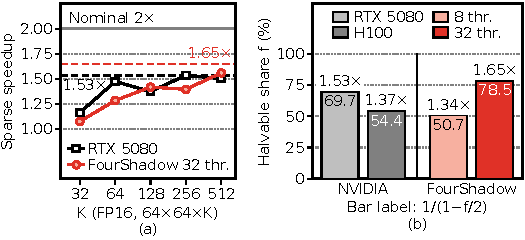
\includegraphics[width=\columnwidth]
    {hpca2027-latex-template/fig/paper_sparse_nvidia_compare_ab.pdf}
    \caption{Warp-level 2:4 sparsity on FourShadow and NVIDIA GPUs, FP16,
    $64{\times}64{\times}K$: (a)~dense-over-sparse speedup against $K$, dashed
    lines the bounds $1/(1-f/2)$; (b)~halvable share $f$, with the bound as bar label.}
    \label{fig:sparse_nvidia}
\end{figure}

\begin{figure}[t]
    \centering
    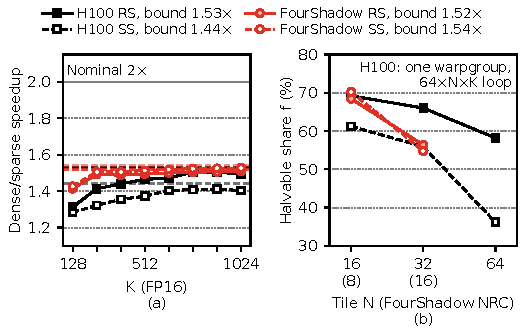
\includegraphics[width=\columnwidth]
    {hpca2027-latex-template/fig/sparse_wg_halvable.pdf}
    \caption{Warp-group MMA with 2:4 sparsity on FourShadow and an H100, FP16:
    (a)~speedup against $K$, dashed lines the bounds; (b)~halvable share $f$
    against the tile width $N$.}
    \label{fig:sparse_wg_halvable}
\end{figure}

\subsubsection{Only Part of the Sparse Cost Halves}\label{sec:eval_sparse_halves}

For the $64{\times}64{\times}K$ FP16 GEMM of Fig.~\ref{fig:sparse_nvidia}(a), the dense-over-sparse speedup rises with $K$ but stays below 2$\times$: from 1.16$\times$ at $K{=}32$ to 1.50$\times$ at $K{=}512$ on the RTX 5080, and from 1.07$\times$ to 1.56$\times$ on FourShadow at 32 threads per warp. Over issue widths of 1, 2 and 4 with 4 or 16 warps, at 8 and 32 threads, FourShadow stays below 2$\times$: its maximum is 1.92$\times$, for the INT8 $128{\times}128{\times}1024$ GEMM at (IW-1, NW-16) and 32 threads. \phantomsection\label{sec:large_halves}At $256{\times}256{\times}K$ and $512{\times}512{\times}K$ the maximum is 1.79$\times$ and 1.77$\times$.

We fit the cycles of each $K$ sweep as $C_{\mathrm{dense}} = c + (a+d)K$ and $C_{\mathrm{sparse}} = c' + (a/2+d)K$, where $a$ is the per-$K$ cost that 2:4 sparsity is assumed to halve exactly, and $d$ the per-$K$ cost that it leaves unchanged ($c$ and $c'$ do not depend on $K$). The fitted slopes $s_{\mathrm{dense}} = a+d$ and $s_{\mathrm{sparse}} = a/2+d$ give the halvable share $f = a/(a+d) = 2(1 - s_{\mathrm{sparse}}/s_{\mathrm{dense}})$, and as $K$ grows the speedup approaches the bound $1/(1-f/2) = s_{\mathrm{dense}}/s_{\mathrm{sparse}}$. For FP16, $f$ is 69.7\% on the RTX 5080 and 78.5\% on FourShadow at 32 threads, which gives the dashed lines of Fig.~\ref{fig:sparse_nvidia}(a) at 1.53$\times$ and 1.65$\times$. Here $a$ contains the tensor-core math and the $A$ load, which halve together, and $d$ the $B$ load and the metadata. At 8 threads per warp FourShadow's instruction counts confirm this split: the halved $A$-fragment loads and WMMA micro-ops predict $a$ within 2.2\%.

Sparsity is faster in each of the 17 shapes measured on both FourShadow and the RTX 5080, and the two speedups differ by a median of 6.2\% at 32 threads and 9.0\% at 8 threads. Only the FP16 fits are valid on the RTX 5080: the TF32 fit has a negative dense intercept, $-$50,243 cycles, and the INT8 fit has only four values of $K$, so Fig.~\ref{fig:sparse_nvidia}(b) shows FP16 alone. On an H100 the same $64{\times}64{\times}K$ FP16 GEMM gives a halvable share of 54.4\% and a bound of 1.37$\times$, and FourShadow at 8 threads per warp gives 50.7\% and 1.34$\times$. The share therefore differs between GPU generations and between FourShadow configurations, while the cost structure, a per-$K$ cost of which sparsity halves only a part, holds on all of them. On the NVIDIA GPUs this reading of $a$ and $d$ is an interpretation: no counter at the in-kernel region separates them. For warp-group MMA on the H100 the data type does not matter: TF32, FP16, BF16 and E4M3 give the same issue intervals and latencies within 0.042 cycles.

\answerbox{Answer \#2 for Q1}{2:4 sparsity halves only part of the per-$K$ cost of a warp-level tensor-core GEMM, so its speedup stays below 2$\times$ and depends on the size of that halvable part: for FP16 it is 69.7\% on the RTX 5080 (bound 1.53$\times$) and 54.4\% on the H100 (1.37$\times$).}

\subsubsection{The Halvable Share Falls as the Warp-Group Tile Widens}\label{sec:eval_sparse_wg}

With identical staging in the dense and sparse kernels, 2:4 sparsity speeds up FourShadow's warp-group GEMM by 1.41--1.53$\times$ and the H100's by 1.28--1.51$\times$, below 2$\times$ at every $K$ (Fig.~\ref{fig:sparse_wg_halvable}(a)). \phantomsection\label{sec:large_wg}The same pair at $256{\times}256{\times}K$ and $512{\times}512{\times}K$ gains 1.39--1.53$\times$, and its halvable shares, under synchronous or double-buffered DXA staging, stay within 1 point of those at $128{\times}128{\times}K$. \phantomsection\label{sec:skinny_sparse}On skinny shapes FourShadow's sparsity speedup is 1.42--1.54$\times$, and 1.51--1.53$\times$ on the decode-like tall $128{\times}32{\times}1536$ GEMM.
% Source (skinny): skinny.json families.128 claim F8.1 (t32 1.44-1.53, t64 1.43-1.54, w64 1.42-1.53; SKINNY.md 5.4 row 9) and SKINNY.md 5.3 finding 7 (t32, K 1536: 1.51-1.53); rechecked from runs-bfix2-skinny-128-f8.jsonl (dense / res, 32 thr., NRC 8, RS+SS) on 2026-10-11.
FourShadow runs the $128{\times}128{\times}K$ GEMM at (IW-4, NW-4), 32 threads per warp and $\mathit{NRC}{=}8$, timed in total kernel cycles, with the metadata loaded once before the loop and the warps copying $A$ and $B$ into shared memory before each warp-group MMA (synchronous staging); its dense and sparse kernels differ only in the length of $A$ per $K$ step and in the MMA instruction. The H100 runs one warpgroup's $64{\times}16{\times}K$ loop, the tile of equal $N$ (Section~\ref{sec:method_hw}) and pipelines its operand staging, overlapping it with the warp-group MMA. Both speedups rise with $K$ toward their bounds.

The halvable-share model of Section~\ref{sec:eval_sparse_halves} fits these sweeps as well, with positive intercepts and seven (H100) or eight (FourShadow) values of $K$; at $N{=}16$ its bounds are the dashed lines of Fig.~\ref{fig:sparse_wg_halvable}(a), 1.44--1.54$\times$.

On both machines $f$ falls as the tile widens (Fig.~\ref{fig:sparse_wg_halvable}(b)): in the H100's pipelined loop from 69.2 to 58.2\% in RS mode and from 61.2 to 36.2\% in SS mode between $N{=}16$ and 64, and on FourShadow with synchronous staging from 68.4 to 56.4\% and from 70.2 to 54.8\% between $N{=}16$ and 32. Sparsity halves $A$ but not $B$, and $B$ grows with $N$ while $A$ does not. On the H100 this follows from the operand sizes: per $K$, a sparse instruction halves the math and the bytes of the 64-row $A$ but carries the same bytes of the $N$-column $B$. On FourShadow the instruction counts show it: sparsity halves the $A$ copy and the micro-ops of the warp-group MMA, while the $B$ copy is the same in both kernels and doubles from $\mathit{NRC}{=}8$ to 16; in SS mode at 32 threads these two halved parts account for the fitted $a$ within 1\%.

The same parts halve in RS and SS mode on both machines, the math and $A$ but not $B$, yet in this loop the H100 gains more in RS than in SS mode, by 8 to 22 points of $f$, while FourShadow gains about equally in both, within 2 points. On FourShadow the share also depends on how exposed the staging of $A$ is: at $N{=}16$ it is 68--70\% with synchronous staging and 27--31\% with double-buffered DXA staging, which hides the transfer of $A$ so that only the micro-ops of the warp-group MMA halve; the two machines therefore agree in how $f$ falls with $N$, not in its size.

\answerbox{Answer \#3 for Q1}{2:4 sparsity halves the $A$ operand of a warp-group MMA GEMM but not $B$, which grows with the tile width $N$, so the halvable share falls as the tile widens, on both the H100 (pipelined loop) and FourShadow.}

\subsection{FPGA Design Flow}\label{sec:eval_fpga}

We implement FourShadow on an AMD Alveo U55C with 16\,GB HBM2 at
200\,MHz. The evaluated system contains
one core with sixteen 8-thread warps, an issue width of four, and four
8-lane Ten-Four\cite{rout2026tenfouropensourcefuseddot} blocks supporting FP16 inputs and FP32
accumulation, WGMMA, 2K-wide FEDP, and 2:4 structured sparsity. Table~\ref{tab:fpga-config} lists the full configuration and end-to-end workloads. The sparse modes prune only the weights, once and offline before the timed run, by one-shot magnitude 2:4 pruning. The configuration of this FPGA build, in particular the 8-thread and single-core parameters, is limited by the resources on the U55C FPGA board. Table~\ref{tab:tcu-parts} shows the hierarchical utilization overhead of each FourShadow extended unit.
Of the post-route LUT utilization of the fully enabled Vortex core,
including its first-level caches, local memory and DXA engine, the 4-block TCU
takes 40.6\%, the issue stage and front end 23.1\%, the FPU 22.7\%,
memory (first-level caches and local memory) 5.4\%, the ALU 3.2\%, the
DXA engine 2.5\%, the LSU 1.4\% and the SFU 0.9\%.

\begin{table}
  \centering
  \caption{FPGA build configuration and end-to-end workloads.}
  \label{tab:fpga-config}
  \footnotesize
  \setlength{\tabcolsep}{3pt}
  \begin{tabular}{@{}lr|lr@{}}
  \toprule
  \textbf{Cores}                & 1           & \textbf{L1 I-cache}      & 16\,KB, 4-way \\
  \textbf{Warps$\times$threads} & 16$\times$8 & \textbf{L1 D-cache}      & 16\,KB, 4-way, WB \\
  \textbf{Issue width}          & 4           & \textbf{Cache line size} & 64\,B \\
  \textbf{ALU / FPU blocks}     & 4 / 4       & \textbf{Local memory}    & 16\,KB, 8 banks \\
  \textbf{SFU / LSU blocks}     & 1 / 1       & \textbf{L2 / L3}         & Disabled \\
  \textbf{TCU blocks}           & 4, FEDP2K   &                          & \\
\midrule
% TODO(ispass): the end-to-end workload settings below were filled in by the co-authors and are not yet checked against the FPGA run sources (Llama decode token count, attention/FlashAttention/CNN/NeRF/MoE settings).
\multicolumn{4}{@{}p{\linewidth}@{}}{\textbf{End-to-end workloads} (Fig.~\ref{fig:e2e_fpga}): CNN, 2D convolution (in/out channels 128/128, height 64, width 64, kernel size 3); attention layer with Q/K/V and output projections (512 tokens, hidden dim.\ 1024, 16 heads); FlashAttention (sequence length 4096, head dim.\ 32); Llama-3.2-1B decode (8 tokens, batch 32) and prefill (128-token prompt); NeRF (512 rays, 64 samples); MoE (512 tokens, hidden dim.\ 2048, FFN dim.\ 2048, 8 experts, top-2). All run FP16 inputs with FP32 accumulation.} \\
  \bottomrule
  \end{tabular}
\end{table}

\begin{table}
  \centering
  \caption{Post-route resource breakdown of the fully enabled
  FourShadow TCU on the Alveo U55C.}
  \label{tab:tcu-parts}
  \setlength{\tabcolsep}{5pt}
  \renewcommand{\arraystretch}{1.15}
  \begin{tabular}{@{}lrrrr@{}}
  \toprule
  \textbf{Part} & \textbf{LUT} & \textbf{FF} &
  \textbf{LUTRAM} & \textbf{DSP} \\
  \midrule
  FEDP array ($4\times$)                        & 98\,379 & 32\,441 & 0 & 256 \\
  Lane dispatch                                 & 26\,909 & 6\,776  & 0 & 0   \\
  WGMMA control                                 & 18\,666 & 5\,547  & 0 & 2   \\
  2:4 metadata ($4\times$)                      & 5\,060  & 0       & 4\,096 & 0   \\
  Input queues ($4\times$)                      & 3\,484  & 1\,348  & 680 & 0   \\
  AGU                                           & 1\,782  & 1\,300  & 0 & 0   \\
  Lane gather                                   & 25      & 2\,252  & 0 & 0   \\
  \midrule
  \textbf{TCU total}                            &
  \textbf{154\,305} & \textbf{49\,664} & \textbf{4\,776} & \textbf{258} \\
  \bottomrule
  \end{tabular}
\end{table}

Fig.~\ref{fig:e2e_fpga} shows end-to-end speedups over the dense
warp-level MMA (WMMA) baseline. WGMMA alone reaches 10.28$\times$ for
MoE, 10.18$\times$ for Llama-3.2-1B prefill, 7.76$\times$ for decode,
4.24$\times$ for attention and 3.13$\times$ for CNN, but only
1.71$\times$ for NeRF and 1.05$\times$ for FlashAttention. Sparsity
alone gives at most 1.12$\times$, except 1.51$\times$ for attention;
on top of WGMMA it adds 1.03--1.30$\times$, reaching 12.74$\times$ for
MoE, 12.39$\times$ for prefill and 4.72$\times$ for attention. The
speedups are smaller for workloads whose runtime is not GEMM-dominated,
such as FlashAttention and NeRF. The WMMA baseline loads its operands directly from global memory without DXA, so part of WGMMA's gain is DXA hiding memory latency, as the 50-cycle experiment below shows.
Surprisingly, these end-to-end speedups exceed the single-tile
speedups. This is mainly because the FPGA's memory system has a higher
latency than the simulation model, which omits the FPGA's interconnect and HBM controller. WMMA is sensitive to global memory
latency, whereas WGMMA is less so because it overlaps computation with
data movement from global memory: in RTL simulation, modeling a flat additional 50-cycle delay in the memory controller slows Llama-3.2-1B decode's $512{\times}32{\times}2048$ K/V projection by 1.75$\times$ with WMMA but by only 1.01$\times$ with WGMMA. The FPGA's HBM also has far higher
bandwidth than the simulated memory, but matching the simulator's
bandwidth to it reduces a GEMM's cycle count by at most 9\%.
\begin{figure}
    \centering
    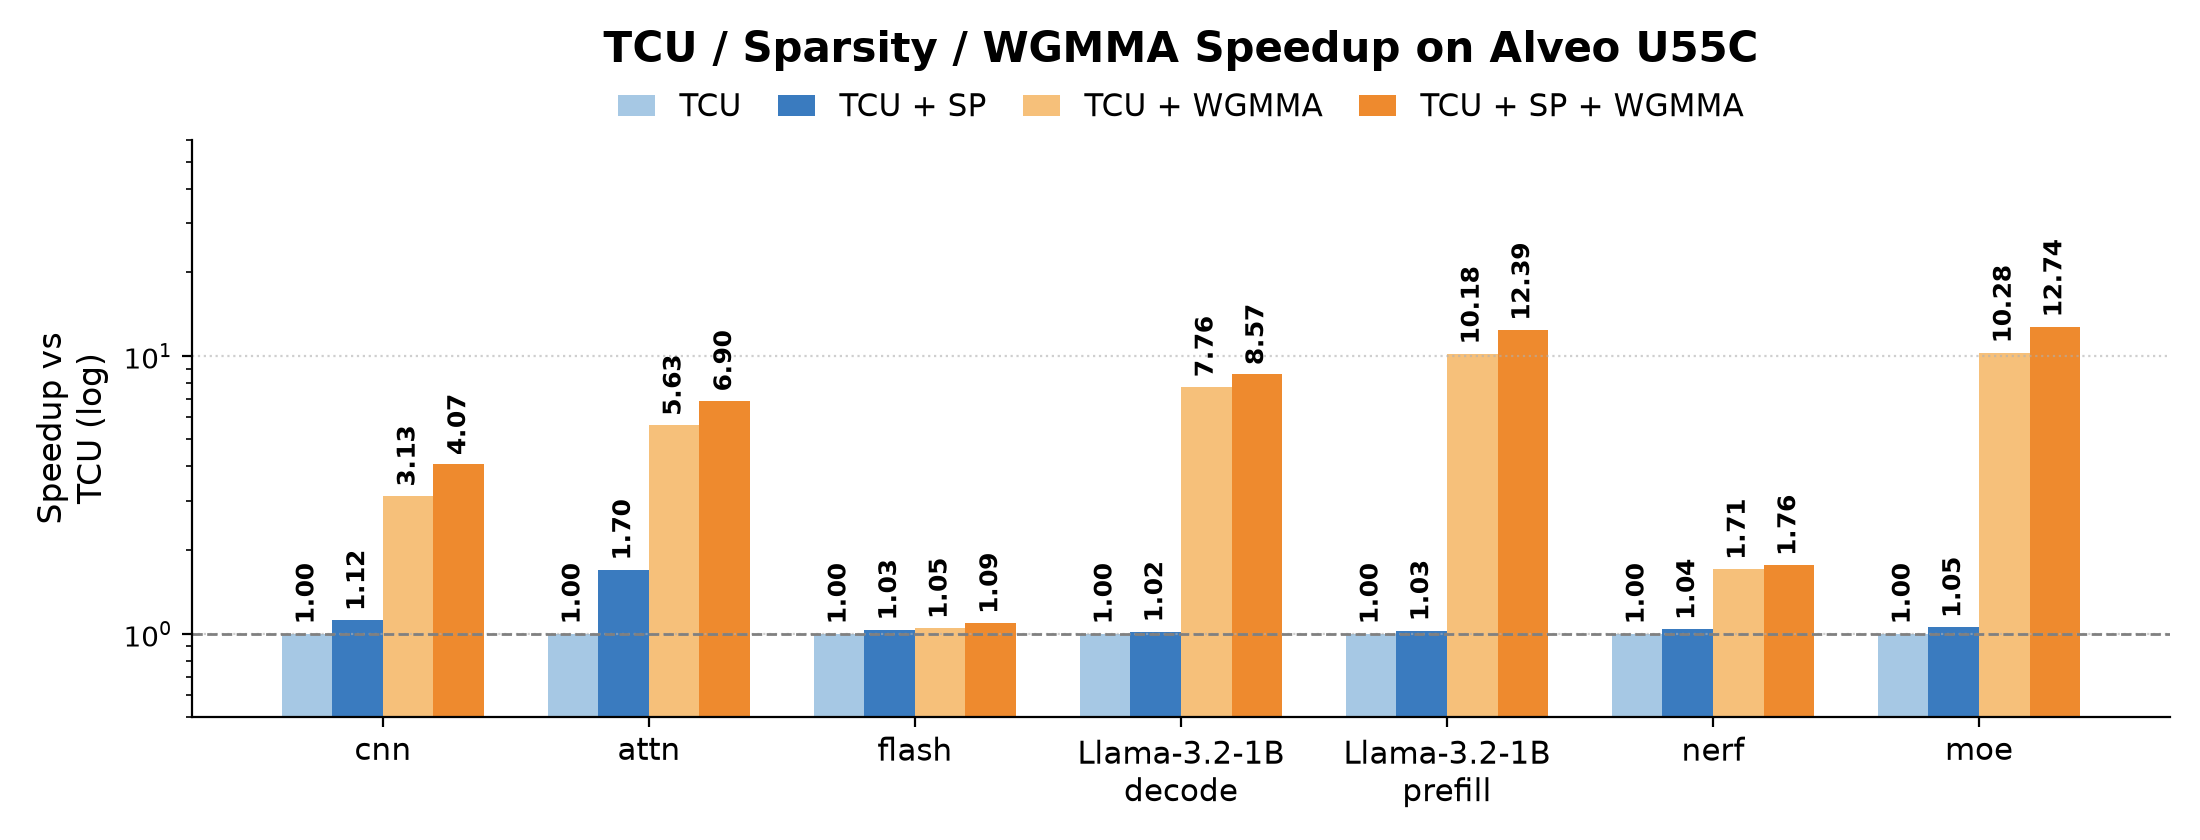
\includegraphics[width=\linewidth]
    {hpca2027-latex-template/fig/fpga_e2e.png}
    \caption{End-to-end FPGA speedup over the dense TCU baseline on
    the Alveo U55C at 200\,MHz.}
    \label{fig:e2e_fpga}
\end{figure}

\subsection{ASIC Design Flow}\label{sec:eval_asic}

\subsubsection{ASIC Synthesis and Timing}
% Source: FourShadow core synthesis report (Vortex master @ 39e76eefa), tables copied to fig/src/asic_runs.csv and asic_e3d_breakdown.csv.
We synthesize the whole core (one cluster with one core, including its L1 caches, local memory and DXA) with Synopsys Design Compiler X-2025.06-SP1 on ASAP7 7.5-track LVT cells (TT corner) and SRAM macros at 1\,GHz. ASAP7 has no dual-ported SRAM, so the register file is built from flip-flops, which inflates its area. We synthesize a threads-per-warp sweep (16 warps, $\mathit{IW}{=}1$) and a feature ladder ($\mathit{NT}{=}\mathit{NW}{=}\mathit{IW}{=}4$) that adds the extensions one at a time. All eight cores meet 1\,GHz; the TCU's FEDP pipeline is critical only at 4, 8 and 32 threads, so no extension limits the clock.

\begin{figure}
    \centering
    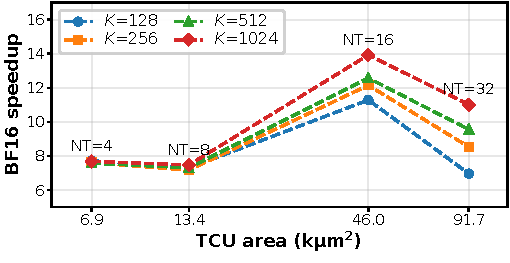
\includegraphics[width=\linewidth,trim=0 5 0 0,clip]
    {hpca2027-latex-template/fig/asic_nt_area_speedup.pdf}
    \caption{BF16 SGEMM speedup over scalar FP32 against TCU area
    across threads per warp (16 warps, $\mathit{IW}{=}1$).}
    \label{fig:asic_nt}
\end{figure}

\subsubsection{Threads/Warp Area--Performance Tradeoff}
The TCU grows by 1.95$\times$, 3.43$\times$ and 2.00$\times$ from 4 to 8, 16 and 32 threads (Fig.~\ref{fig:asic_nt}): each step doubles the FEDP units, and from 8 to 16 threads each unit's dot product doubles too (Eqs.~(\ref{eq:block_cap})--(\ref{eq:block_tc})). The BF16 speedup of Fig.~\ref{fig:threads_sweep}(a) follows only the latter: it falls by 3--6\% from 4 to 8 threads, rises by 1.55--1.86$\times$ at 16, and falls by 21--38\% at 32 while the TCU doubles to 91.7\,k$\mu$m$^2$. Sixteen threads thus give the highest speedup, and 32 spend twice the area for less. The TCU is 4.2--9.6\% of the core, which grows from 0.165 to 0.960\,mm$^2$, largely in the flip-flop register file. The TCU's share depends on the platform and configuration: 4.2--9.6\% of this core at $\mathit{IW}{=}1$ with 16 warps, where the flip-flop register file dominates; 8.0\% of the full-featured core at $\mathit{NT}{=}\mathit{NW}{=}\mathit{IW}{=}4$, where the flip-flop L1 data cache dominates; and 40.6\% of the FPGA core's LUTs (Section~\ref{sec:eval_fpga}), which leave out memories mapped to block RAM.

\subsubsection{Issue-Width Area--Performance Tradeoff}
TCU area grows almost linearly with issue width (Fig.~\ref{fig:iw_area_scaling}), from 58.6 to 115.6 and 230.6\,k$\mu$m$^2$ at $\mathit{IW}{=}1$, 2 and 4, while the speedup reaches only 1.37--1.41$\times$ and 1.67--1.71$\times$; $\mathit{IW}{=}8$, at an estimated 455--462\,k$\mu$m$^2$, gains just 1.70--1.81$\times$. $\mathit{IW}{=}4$ is thus the practical optimum, beyond which the core's instruction front end (Section~\ref{sec:eval_iw}), not arithmetic capacity, limits a wider warpgroup.
\begin{figure}
    \centering
    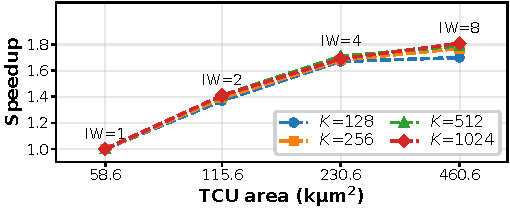
\includegraphics[width=\linewidth,trim=0 5 0 0,clip]
    {hpca2027-latex-template/fig/iw_area_speedup_short.pdf}
    \caption{WGMMA speedup over $\mathit{IW}{=}1$ against TCU
    area at $\mathit{NT}{=}16$.}
    \label{fig:iw_area_scaling}
\end{figure}

\begin{figure}
    \centering
    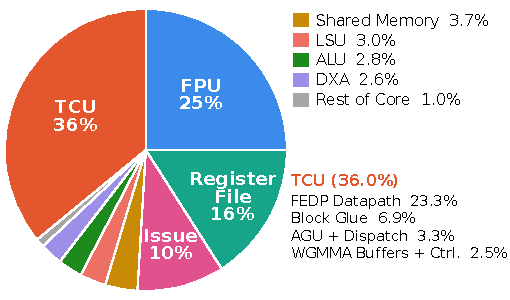
\includegraphics[width=0.9\linewidth]{hpca2027-latex-template/fig/asic_area_breakdown.pdf}
    \caption{Sub-core area breakdown of a full-featured FourShadow TCU}
    \label{fig:asic_breakdown}
\end{figure}

\subsubsection{Area Cost of the Tensor-Core Extensions}
Fig.~\ref{fig:asic_breakdown} illustrates the ASIC cell area breakdown of a full FourShadow extended Vortex SIMT core. Key findings from adding each extension include:
\begin{itemize}
    \item \textbf{2:4 sparsity} adds 1,745\,$\mu$m$^2$ (10\%) to the TCU for the metadata SRAM and the gather logic that selects the kept $B$ values; the core grows by 0.4\%
    \item \textbf{Warp-group MMA with DXA} adds 11,419\,$\mu$m$^2$ (3.9\%) and 3.2\% power, of which the DXA engine is 9,285\,$\mu$m$^2$ and the TCU's tile buffers and control 1,571\,$\mu$m$^2$.
    \item \textbf{The 2K-wide FEDP} grows the TCU by 34\% (6,254\,$\mu$m$^2$), 2.1\% of the core, for 0.8\% more power.
\end{itemize}

%\subsection{Cluster-Level Matrix Unit Integration}
%Virgo~\cite{kim2025virgo} explored a complementary direction by physically disaggregating the matrix unit from individual SIMT cores and placing a larger systolic array at the cluster level. By drawing operands directly from shared memory, Virgo increases operation granularity, improves data reuse, and reduces instruction-processing energy. Evaluations show substantial power and energy reductions compared with core-coupled Ampere- and Hopper-style designs. In contrast to Virgo’s approach of moving the matrix unit outside the SIMT core, FourShadow remains within the core-coupled, inner-product based Tensor Core model and explores its internal design space, rather than changing the unit’s placement in the hierarchy.

\section{Conclusion}

In this work, we presented \textit{FourShadow}, an open-source, synthesizable exploration framework built on the RISC-V Vortex GPGPU to systematically analyze SIMT Tensor Core microarchitectural scaling. By sweeping architectural parameters across ASIC synthesis (ASAP7 7\,nm), FPGA prototyping (AMD Alveo U55C), and cycle-accurate SIMT simulation, we demystified critical hardware trade-offs across the SIMT hierarchy.

%\begin{enumerate}
%    \item \textit{SIMT Hierarchy Scaling:} Tensor Core scaling is non-monotonic with warp width. A 16-thread configuration ($NT=16$) consistently yields the optimal area--performance Pareto frontier, achieving up to $27.46\times$ speedup over scalar execution for FP8. Furthermore, scaling issue width beyond $IW=4$ yields diminishing returns as non-TCU execution and operand delivery overheads dominate.
%    \item \textit{Datapath and Operand Staging:} Expanding the arithmetic datapath to a $2K$-wide FEDP reduces execution cycles by 28--30\%, absorbing minor pipeline latency increases. Conversely, offloading small control descriptors from registers into TCU-local SRAM introduces an unnecessary 1.2--6.5\% cycle penalty due to added synchronization and memory traffic.
%    \item \textit{Sparsity and Workload Mapping:} Achievable speedups from 2:4 structured sparsity ($2.21$--$2.35\times$ for WGMMA) depend on whether physical compressed mappings preserve full FEDP array utilization. When aligned with application memory intensity, combined WGMMA and sparse acceleration achieve end-to-end speedups of $9.6\times$ and $2.3\times$ for Llama~2 prefill and decode, respectively, and up to $26.82\times$ on compute-heavy NeRF workloads.
%\end{enumerate}

Beyond core-level insights, FourShadow serves as a robust substrate for holistic, open-source microarchitectural design space exploration (DSE). Moving forward, we plan to extend the framework in two key directions: (1)~integrating Distributed Shared Memory (DSMEM) mechanisms to enable multi-core warpgroups to exchange and broadcast matrix tiles directly across local SRAMs without hitting L2 cache bottlenecks and (2)~broadening microarchitectural DSE to explore emerging low-precision formats (e.g., NVFP4, MXFP), novel warp scheduling heuristics, and custom hardware--software co-design extensions.

%%%%%%% -- PAPER CONTENT ENDS -- %%%%%%%%


%%%%%%%%% -- BIB STYLE AND FILE -- %%%%%%%%
\bibliographystyle{IEEEtranS}
\bibliography{refs}
%%%%%%%%%%%%%%%%%%%%%%%%%%%%%%%%%%%%

\section*{Appendix}

Portions of this submission were prepared with the assistance of large language models (Anthropic Claude and Open AI GPT), used as a coding assistant under author direction. Also, the figures in the evaluation part, the organization of the evaluation section were assisted by models.


\end{document}
